%% ECON 282E -- Session 7, Deck A3: Training
%% Sources: AI-ECON Lec03_T3_Training_Backprop.tex, carried WHOLE (28 frames);
%% Feng & Miao, "AI for Economists" (Book1), ch.9 sections 9.3-9.4;
%% Quant_Macro Lec.5 "Toy Example: Forward Pass" / "Backpropagation Step".
%% CARRY-FORWARD OBLIGATION (build plan, 2026-09-17): this deck discharges the
%% S04_A3 callbacks on conjugate gradient and stochastic gradient descent.  It
%% CITES ledger keys cg_steps, optimizer_memory, sgd_trajectory and
%% sgd_dimension from tools/figures/s04_numbers.json; it does not recompute them.
%% Its own numbers come from tools/figures/s07_numbers.json, keys
%% "backprop_sigmoid", "backprop_worked", "epoch_tradeoff", "regularization",
%% "activations".  Figures copied into ./figures/ from Lec03_ML_for_Macro/pic/
%% (renamed to lowercase: check_course.py does not resolve a .PNG extension).

%% ECON 282E -- Foundations of Macroeconomics (UC Riverside, Fall 2026)
%% Shared Beamer preamble for every deck in slides/S01 ... slides/S10.
%%
%% Usage (a deck lives in slides/S0X/ and is compiled from that folder):
%%   %% ECON 282E -- Foundations of Macroeconomics (UC Riverside, Fall 2026)
%% Shared Beamer preamble for every deck in slides/S01 ... slides/S10.
%%
%% Usage (a deck lives in slides/S0X/ and is compiled from that folder):
%%   %% ECON 282E -- Foundations of Macroeconomics (UC Riverside, Fall 2026)
%% Shared Beamer preamble for every deck in slides/S01 ... slides/S10.
%%
%% Usage (a deck lives in slides/S0X/ and is compiled from that folder):
%%   \input{../preamble/course_preamble.tex}
%%   \decktitle{1}{A1}{Who I Am \& Why This Course}{September 24, 2026}
%%   \begin{document}
%%   \makedecktitle
%%   ...
%%
%% Adapted from Courses/AI-ECON-2026/source/shared_preamble.tex (Metropolis theme,
%% concept/caution/example/takeaway boxes, \sectiondivider). Changes for this course:
%%   * course title block (\decktitle / \makedecktitle) instead of \makebeamertitle
%%   * \zh{...} typesets Chinese (book titles) under pdflatex via CJKutf8
%%   * researchbox for the "Research in the wild" frames
%%   * section pages off; TikZ libraries and the course map loaded here
%% Build with pdflatex only (two passes); tools/build_slides.py does this for you.

\documentclass[10pt,english,aspectratio=169]{beamer}

\usepackage[T1]{fontenc}
\usepackage{textcomp}
\usepackage[utf8]{inputenc}
\usepackage{babel}
\usepackage{CJKutf8}

\usepackage{amsmath, amssymb, amsthm, graphicx}
\usepackage{booktabs, multirow, tabularx}
\usepackage{tikz}
\usetikzlibrary{positioning,arrows.meta,shapes,calc,fit,backgrounds}
\usepackage{pgfplots}
\pgfplotsset{compat=1.16}
\usepackage[most]{tcolorbox}
\tcbuselibrary{skins, breakable}
\usepackage{listings}
\usepackage{xcolor}

\lstset{
  basicstyle=\ttfamily\small,
  keywordstyle=\color{blue!80!black}\bfseries,
  commentstyle=\color{green!50!black}\itshape,
  stringstyle=\color{orange!80!black},
  backgroundcolor=\color{gray!8},
  frame=single,
  rulecolor=\color{gray!40},
  breaklines=true,
  showstringspaces=false,
  numbers=none,
}

\usetheme{metropolis}
\usefonttheme{professionalfonts}
\metroset{sectionpage=none}

\definecolor{LightGray}{RGB}{230,230,230}
\definecolor{RedTitle}{RGB}{0,0,200}
\definecolor{VeryLightGray}{RGB}{245,245,245}
\definecolor{DarkText}{RGB}{0,0,0}
\definecolor{UCRBlue}{RGB}{0,45,106}
\definecolor{UCRGold}{RGB}{241,171,0}

% Stage colours of the course arc (used by the course map and elsewhere)
\colorlet{StageTrunk}{blue!12}
\colorlet{StageBranch}{cyan!14}
\colorlet{StageMachine}{gray!18}
\colorlet{StageWall}{red!14}
\colorlet{StageTools}{orange!20}
\colorlet{StageData}{green!16}
\colorlet{StageAgents}{violet!14}

\hypersetup{bookmarks=false,breaklinks=true,pdfborder={0 0 0},colorlinks=true,
  linkcolor=DarkText,urlcolor=RedTitle}

\setbeamercolor{background canvas}{bg=white}
\setbeamercolor{title}{fg=RedTitle}
\setbeamercolor{frametitle}{bg=VeryLightGray,fg=DarkText}
\setbeamercolor{normal text}{fg=DarkText}
\setbeamercolor{alerted text}{fg=RedTitle}
\setbeamersize{text margin left=5mm, text margin right=5mm}
\addtobeamertemplate{frametitle}{}{\vspace{-0.5em}}

\setbeamertemplate{navigation symbols}{}
\setbeamertemplate{footline}{%
  \hspace{5mm}{\usebeamerfont{page number in head/foot}\color{black!45}%
  ECON 282E \,$\cdot$\, \insertshortdeck}\hfill%
  \usebeamercolor[fg]{page number in head/foot}%
  \usebeamerfont{page number in head/foot}%
  \insertframenumber\,/\,\inserttotalframenumber\kern1em\vskip2pt%
}

% ---------------------------------------------------------------------------
% Chinese text under pdflatex (book titles etc.)
\newcommand{\zh}[1]{\begin{CJK*}{UTF8}{gbsn}#1\end{CJK*}}

% ---------------------------------------------------------------------------
% Deck title block
%   \decktitle{session}{deck id}{title}{date}
\newcommand{\insertshortdeck}{}
\newcommand{\decksession}{}
\newcommand{\deckid}{}
\newcommand{\decktitletext}{}
\newcommand{\deckdate}{}
\newcommand{\decktitle}[4]{%
  \renewcommand{\decksession}{#1}%
  \renewcommand{\deckid}{#2}%
  \renewcommand{\decktitletext}{#3}%
  \renewcommand{\deckdate}{#4}%
  \renewcommand{\insertshortdeck}{Session #1 \,$\cdot$\, Deck #1.#2}%
  \title{#3}%
  \author{Zhigang Feng}%
  \date{#4}%
}
\newcommand{\makedecktitle}{%
  \begin{frame}[plain,noframenumbering]
    \begin{tikzpicture}[remember picture,overlay]
      \fill[UCRBlue] (current page.north west) rectangle ([yshift=-0.55cm]current page.north east);
      \fill[UCRGold] ([yshift=-0.55cm]current page.north west) rectangle ([yshift=-0.62cm]current page.north east);
      \node[anchor=west, text=white, font=\small\bfseries] at ([xshift=5mm,yshift=-0.275cm]current page.north west)
        {ECON 282E \,$\cdot$\, Foundations of Macroeconomics};
      \node[anchor=east, text=white, font=\small] at ([xshift=-5mm,yshift=-0.275cm]current page.north east)
        {UC Riverside \,$\cdot$\, Fall 2026};
    \end{tikzpicture}
    \vspace*{1.1cm}
    {\usebeamerfont{title}\color{black!55}\large Session \decksession\ \,$\cdot$\, Deck \decksession.\deckid\par}
    \vspace{0.25cm}
    {\usebeamerfont{title}\color{RedTitle}\LARGE\bfseries \decktitletext\par}
    \vspace{0.7cm}
    {\large Zhigang Feng\par}
    \vspace{0.15cm}
    {\color{black!65}\deckdate\par}
    \vfill
    {\footnotesize\itshape\color{black!55}Build it on paper $\;\to\;$ solve it on the machine $\;\to\;$ push it to the frontier with AI\par}
  \end{frame}}

% ---------------------------------------------------------------------------
% Section divider (plain frame, not counted)
\newcommand{\sectiondivider}[2]{%
\begin{frame}[plain,noframenumbering]
\begin{center}
\vfill
{\Large\textbf{#1}\par}
\vspace{0.35cm}
{\normalsize #2\par}
\vfill
\end{center}
\end{frame}
}

% ---------------------------------------------------------------------------
% Boxes
\newtcolorbox{conceptbox}[1][]{colback=blue!3, colframe=RedTitle!55, boxrule=0.35mm,
  arc=1mm, left=2mm, right=2mm, top=1mm, bottom=1mm, #1}
\newtcolorbox{cautionbox}[1][]{colback=red!3, colframe=red!50!black, boxrule=0.35mm,
  arc=1mm, left=2mm, right=2mm, top=1mm, bottom=1mm, #1}
\newtcolorbox{examplebox}[1][]{colback=green!3, colframe=green!45!black, boxrule=0.35mm,
  arc=1mm, left=2mm, right=2mm, top=1mm, bottom=1mm, #1}
\newtcolorbox{takeawaybox}[1][]{colback=VeryLightGray, colframe=RedTitle!55, boxrule=0.35mm,
  arc=1mm, left=2mm, right=2mm, top=1mm, bottom=1mm, #1}
\newtcolorbox{researchbox}[1][]{enhanced, colback=violet!4, colframe=violet!60!black,
  boxrule=0.35mm, arc=1mm, left=2mm, right=2mm, top=1mm, bottom=1mm,
  fonttitle=\bfseries\small, title={Research in the wild}, #1}

\newcommand{\compacttables}{\renewcommand{\arraystretch}{1.15}}
\newcommand{\src}[1]{{\tiny\color{black!55}#1}}

% ---------------------------------------------------------------------------
\input{../preamble/course_map.tex}

%%   \decktitle{1}{A1}{Who I Am \& Why This Course}{September 24, 2026}
%%   \begin{document}
%%   \makedecktitle
%%   ...
%%
%% Adapted from Courses/AI-ECON-2026/source/shared_preamble.tex (Metropolis theme,
%% concept/caution/example/takeaway boxes, \sectiondivider). Changes for this course:
%%   * course title block (\decktitle / \makedecktitle) instead of \makebeamertitle
%%   * \zh{...} typesets Chinese (book titles) under pdflatex via CJKutf8
%%   * researchbox for the "Research in the wild" frames
%%   * section pages off; TikZ libraries and the course map loaded here
%% Build with pdflatex only (two passes); tools/build_slides.py does this for you.

\documentclass[10pt,english,aspectratio=169]{beamer}

\usepackage[T1]{fontenc}
\usepackage{textcomp}
\usepackage[utf8]{inputenc}
\usepackage{babel}
\usepackage{CJKutf8}

\usepackage{amsmath, amssymb, amsthm, graphicx}
\usepackage{booktabs, multirow, tabularx}
\usepackage{tikz}
\usetikzlibrary{positioning,arrows.meta,shapes,calc,fit,backgrounds}
\usepackage{pgfplots}
\pgfplotsset{compat=1.16}
\usepackage[most]{tcolorbox}
\tcbuselibrary{skins, breakable}
\usepackage{listings}
\usepackage{xcolor}

\lstset{
  basicstyle=\ttfamily\small,
  keywordstyle=\color{blue!80!black}\bfseries,
  commentstyle=\color{green!50!black}\itshape,
  stringstyle=\color{orange!80!black},
  backgroundcolor=\color{gray!8},
  frame=single,
  rulecolor=\color{gray!40},
  breaklines=true,
  showstringspaces=false,
  numbers=none,
}

\usetheme{metropolis}
\usefonttheme{professionalfonts}
\metroset{sectionpage=none}

\definecolor{LightGray}{RGB}{230,230,230}
\definecolor{RedTitle}{RGB}{0,0,200}
\definecolor{VeryLightGray}{RGB}{245,245,245}
\definecolor{DarkText}{RGB}{0,0,0}
\definecolor{UCRBlue}{RGB}{0,45,106}
\definecolor{UCRGold}{RGB}{241,171,0}

% Stage colours of the course arc (used by the course map and elsewhere)
\colorlet{StageTrunk}{blue!12}
\colorlet{StageBranch}{cyan!14}
\colorlet{StageMachine}{gray!18}
\colorlet{StageWall}{red!14}
\colorlet{StageTools}{orange!20}
\colorlet{StageData}{green!16}
\colorlet{StageAgents}{violet!14}

\hypersetup{bookmarks=false,breaklinks=true,pdfborder={0 0 0},colorlinks=true,
  linkcolor=DarkText,urlcolor=RedTitle}

\setbeamercolor{background canvas}{bg=white}
\setbeamercolor{title}{fg=RedTitle}
\setbeamercolor{frametitle}{bg=VeryLightGray,fg=DarkText}
\setbeamercolor{normal text}{fg=DarkText}
\setbeamercolor{alerted text}{fg=RedTitle}
\setbeamersize{text margin left=5mm, text margin right=5mm}
\addtobeamertemplate{frametitle}{}{\vspace{-0.5em}}

\setbeamertemplate{navigation symbols}{}
\setbeamertemplate{footline}{%
  \hspace{5mm}{\usebeamerfont{page number in head/foot}\color{black!45}%
  ECON 282E \,$\cdot$\, \insertshortdeck}\hfill%
  \usebeamercolor[fg]{page number in head/foot}%
  \usebeamerfont{page number in head/foot}%
  \insertframenumber\,/\,\inserttotalframenumber\kern1em\vskip2pt%
}

% ---------------------------------------------------------------------------
% Chinese text under pdflatex (book titles etc.)
\newcommand{\zh}[1]{\begin{CJK*}{UTF8}{gbsn}#1\end{CJK*}}

% ---------------------------------------------------------------------------
% Deck title block
%   \decktitle{session}{deck id}{title}{date}
\newcommand{\insertshortdeck}{}
\newcommand{\decksession}{}
\newcommand{\deckid}{}
\newcommand{\decktitletext}{}
\newcommand{\deckdate}{}
\newcommand{\decktitle}[4]{%
  \renewcommand{\decksession}{#1}%
  \renewcommand{\deckid}{#2}%
  \renewcommand{\decktitletext}{#3}%
  \renewcommand{\deckdate}{#4}%
  \renewcommand{\insertshortdeck}{Session #1 \,$\cdot$\, Deck #1.#2}%
  \title{#3}%
  \author{Zhigang Feng}%
  \date{#4}%
}
\newcommand{\makedecktitle}{%
  \begin{frame}[plain,noframenumbering]
    \begin{tikzpicture}[remember picture,overlay]
      \fill[UCRBlue] (current page.north west) rectangle ([yshift=-0.55cm]current page.north east);
      \fill[UCRGold] ([yshift=-0.55cm]current page.north west) rectangle ([yshift=-0.62cm]current page.north east);
      \node[anchor=west, text=white, font=\small\bfseries] at ([xshift=5mm,yshift=-0.275cm]current page.north west)
        {ECON 282E \,$\cdot$\, Foundations of Macroeconomics};
      \node[anchor=east, text=white, font=\small] at ([xshift=-5mm,yshift=-0.275cm]current page.north east)
        {UC Riverside \,$\cdot$\, Fall 2026};
    \end{tikzpicture}
    \vspace*{1.1cm}
    {\usebeamerfont{title}\color{black!55}\large Session \decksession\ \,$\cdot$\, Deck \decksession.\deckid\par}
    \vspace{0.25cm}
    {\usebeamerfont{title}\color{RedTitle}\LARGE\bfseries \decktitletext\par}
    \vspace{0.7cm}
    {\large Zhigang Feng\par}
    \vspace{0.15cm}
    {\color{black!65}\deckdate\par}
    \vfill
    {\footnotesize\itshape\color{black!55}Build it on paper $\;\to\;$ solve it on the machine $\;\to\;$ push it to the frontier with AI\par}
  \end{frame}}

% ---------------------------------------------------------------------------
% Section divider (plain frame, not counted)
\newcommand{\sectiondivider}[2]{%
\begin{frame}[plain,noframenumbering]
\begin{center}
\vfill
{\Large\textbf{#1}\par}
\vspace{0.35cm}
{\normalsize #2\par}
\vfill
\end{center}
\end{frame}
}

% ---------------------------------------------------------------------------
% Boxes
\newtcolorbox{conceptbox}[1][]{colback=blue!3, colframe=RedTitle!55, boxrule=0.35mm,
  arc=1mm, left=2mm, right=2mm, top=1mm, bottom=1mm, #1}
\newtcolorbox{cautionbox}[1][]{colback=red!3, colframe=red!50!black, boxrule=0.35mm,
  arc=1mm, left=2mm, right=2mm, top=1mm, bottom=1mm, #1}
\newtcolorbox{examplebox}[1][]{colback=green!3, colframe=green!45!black, boxrule=0.35mm,
  arc=1mm, left=2mm, right=2mm, top=1mm, bottom=1mm, #1}
\newtcolorbox{takeawaybox}[1][]{colback=VeryLightGray, colframe=RedTitle!55, boxrule=0.35mm,
  arc=1mm, left=2mm, right=2mm, top=1mm, bottom=1mm, #1}
\newtcolorbox{researchbox}[1][]{enhanced, colback=violet!4, colframe=violet!60!black,
  boxrule=0.35mm, arc=1mm, left=2mm, right=2mm, top=1mm, bottom=1mm,
  fonttitle=\bfseries\small, title={Research in the wild}, #1}

\newcommand{\compacttables}{\renewcommand{\arraystretch}{1.15}}
\newcommand{\src}[1]{{\tiny\color{black!55}#1}}

% ---------------------------------------------------------------------------
%% Course map: the recurring "you are here" slide for ECON 282E.
%% Loaded by course_preamble.tex. Pattern follows AI-ECON-2026 lec01_map.tex, but the map
%% shows the whole ten-session course rather than one lecture.
%%
%%   \CourseMap{s}{label}   s = 1..10 highlights session s and prints "you are here: label"
%%                          (e.g. \CourseMap{1}{1.A2}); earlier sessions get a check mark.
%%   \CourseMap{0}{}        full overview, nothing highlighted.
%%
%% Note: TikZ option lists are comma-split before TeX conditionals run, so every \ifnum
%% below sits outside [...] option lists.

\newcommand{\CourseMap}[2]{%
\begin{center}
\begin{tikzpicture}[
    sess/.style={rectangle, rounded corners=2pt, draw=black!45, minimum width=1.34cm,
        minimum height=1.12cm, text width=1.26cm, align=center, inner sep=1pt},
    stage/.style={font=\tiny\bfseries, text=black!70},
]
  \foreach \i/\d/\t/\c in {%
      1/Sep 24/Intro \\ Growth/StageTrunk,
      2/Oct 1/HA $\cdot$ OLG \\ Policy/StageBranch,
      3/Oct 8/Num.\ DP \\ Python/StageMachine,
      4/Oct 15/Numerics \\ I/StageMachine,
      5/Oct 22/Numerics \\ II/StageMachine,
      6/Oct 29/The wall \\ \textbf{Midterm}/StageWall,
      7/Nov 5/ML \\ Deep nets/StageTools,
      8/Nov 12/RL \\ HA $+$ DL/StageTools,
      9/Nov 19/Text \\ LLMs/StageData,
      10/Dec 3/Agents \\ \textbf{Projects}/StageAgents} {
    \node[sess, fill=\c] (n\i) at ({1.46*(\i-1)}, 0)
      {{\scriptsize\bfseries S\i}\\[-1pt]{\tiny\color{black!60}\d}\\[1pt]{\tiny \t}};
    \ifnum\i<#1
      \node[font=\scriptsize, text=green!45!black] at ([xshift=-2.5mm,yshift=-2.2mm]n\i.north east) {$\checkmark$};
    \fi
    \ifnum\i=#1
      \draw[RedTitle, very thick, rounded corners=2pt]
        ([xshift=-0.6mm,yshift=-0.6mm]n\i.south west) rectangle ([xshift=0.6mm,yshift=0.6mm]n\i.north east);
      % keep the label inside the picture at both ends of the row
      \ifnum\i<3
        \node[font=\scriptsize\bfseries, text=RedTitle, anchor=south west] at ([yshift=1.2mm]n\i.north west)
          {$\blacktriangledown$\,you are here: #2};
      \else\ifnum\i>8
        \node[font=\scriptsize\bfseries, text=RedTitle, anchor=south east] at ([yshift=1.2mm]n\i.north east)
          {you are here: #2\,$\blacktriangledown$};
      \else
        \node[font=\scriptsize\bfseries, text=RedTitle, anchor=south] at ([yshift=1.2mm]n\i.north)
          {you are here: #2\,$\blacktriangledown$};
      \fi\fi
    \fi
  }
  % stage band under the sessions
  \foreach \a/\b/\lab/\c in {1/1/trunk/StageTrunk, 2/2/branches/StageBranch,
      3/5/the machine $\cdot$ classical methods/StageMachine, 6/6/the wall/StageWall,
      7/8/new tools/StageTools, 9/9/new data/StageData, 10/10/colleagues/StageAgents} {
    \fill[\c] ([yshift=-1.5mm]n\a.south west) rectangle ([yshift=-4.6mm]n\b.south east);
    \path ([yshift=-1.5mm]n\a.south west) -- ([yshift=-4.6mm]n\b.south east)
      node[midway, stage] {\lab};
  }
  \node[font=\footnotesize\itshape, text=black!70] at ([yshift=-9.5mm]$(n1.south)!0.5!(n10.south)$)
    {Build it on paper $\;\to\;$ solve it on the machine $\;\to\;$ push it to the frontier with AI};
\end{tikzpicture}
\end{center}
}


%%   \decktitle{1}{A1}{Who I Am \& Why This Course}{September 24, 2026}
%%   \begin{document}
%%   \makedecktitle
%%   ...
%%
%% Adapted from Courses/AI-ECON-2026/source/shared_preamble.tex (Metropolis theme,
%% concept/caution/example/takeaway boxes, \sectiondivider). Changes for this course:
%%   * course title block (\decktitle / \makedecktitle) instead of \makebeamertitle
%%   * \zh{...} typesets Chinese (book titles) under pdflatex via CJKutf8
%%   * researchbox for the "Research in the wild" frames
%%   * section pages off; TikZ libraries and the course map loaded here
%% Build with pdflatex only (two passes); tools/build_slides.py does this for you.

\documentclass[10pt,english,aspectratio=169]{beamer}

\usepackage[T1]{fontenc}
\usepackage{textcomp}
\usepackage[utf8]{inputenc}
\usepackage{babel}
\usepackage{CJKutf8}

\usepackage{amsmath, amssymb, amsthm, graphicx}
\usepackage{booktabs, multirow, tabularx}
\usepackage{tikz}
\usetikzlibrary{positioning,arrows.meta,shapes,calc,fit,backgrounds}
\usepackage{pgfplots}
\pgfplotsset{compat=1.16}
\usepackage[most]{tcolorbox}
\tcbuselibrary{skins, breakable}
\usepackage{listings}
\usepackage{xcolor}

\lstset{
  basicstyle=\ttfamily\small,
  keywordstyle=\color{blue!80!black}\bfseries,
  commentstyle=\color{green!50!black}\itshape,
  stringstyle=\color{orange!80!black},
  backgroundcolor=\color{gray!8},
  frame=single,
  rulecolor=\color{gray!40},
  breaklines=true,
  showstringspaces=false,
  numbers=none,
}

\usetheme{metropolis}
\usefonttheme{professionalfonts}
\metroset{sectionpage=none}

\definecolor{LightGray}{RGB}{230,230,230}
\definecolor{RedTitle}{RGB}{0,0,200}
\definecolor{VeryLightGray}{RGB}{245,245,245}
\definecolor{DarkText}{RGB}{0,0,0}
\definecolor{UCRBlue}{RGB}{0,45,106}
\definecolor{UCRGold}{RGB}{241,171,0}

% Stage colours of the course arc (used by the course map and elsewhere)
\colorlet{StageTrunk}{blue!12}
\colorlet{StageBranch}{cyan!14}
\colorlet{StageMachine}{gray!18}
\colorlet{StageWall}{red!14}
\colorlet{StageTools}{orange!20}
\colorlet{StageData}{green!16}
\colorlet{StageAgents}{violet!14}

\hypersetup{bookmarks=false,breaklinks=true,pdfborder={0 0 0},colorlinks=true,
  linkcolor=DarkText,urlcolor=RedTitle}

\setbeamercolor{background canvas}{bg=white}
\setbeamercolor{title}{fg=RedTitle}
\setbeamercolor{frametitle}{bg=VeryLightGray,fg=DarkText}
\setbeamercolor{normal text}{fg=DarkText}
\setbeamercolor{alerted text}{fg=RedTitle}
\setbeamersize{text margin left=5mm, text margin right=5mm}
\addtobeamertemplate{frametitle}{}{\vspace{-0.5em}}

\setbeamertemplate{navigation symbols}{}
\setbeamertemplate{footline}{%
  \hspace{5mm}{\usebeamerfont{page number in head/foot}\color{black!45}%
  ECON 282E \,$\cdot$\, \insertshortdeck}\hfill%
  \usebeamercolor[fg]{page number in head/foot}%
  \usebeamerfont{page number in head/foot}%
  \insertframenumber\,/\,\inserttotalframenumber\kern1em\vskip2pt%
}

% ---------------------------------------------------------------------------
% Chinese text under pdflatex (book titles etc.)
\newcommand{\zh}[1]{\begin{CJK*}{UTF8}{gbsn}#1\end{CJK*}}

% ---------------------------------------------------------------------------
% Deck title block
%   \decktitle{session}{deck id}{title}{date}
\newcommand{\insertshortdeck}{}
\newcommand{\decksession}{}
\newcommand{\deckid}{}
\newcommand{\decktitletext}{}
\newcommand{\deckdate}{}
\newcommand{\decktitle}[4]{%
  \renewcommand{\decksession}{#1}%
  \renewcommand{\deckid}{#2}%
  \renewcommand{\decktitletext}{#3}%
  \renewcommand{\deckdate}{#4}%
  \renewcommand{\insertshortdeck}{Session #1 \,$\cdot$\, Deck #1.#2}%
  \title{#3}%
  \author{Zhigang Feng}%
  \date{#4}%
}
\newcommand{\makedecktitle}{%
  \begin{frame}[plain,noframenumbering]
    \begin{tikzpicture}[remember picture,overlay]
      \fill[UCRBlue] (current page.north west) rectangle ([yshift=-0.55cm]current page.north east);
      \fill[UCRGold] ([yshift=-0.55cm]current page.north west) rectangle ([yshift=-0.62cm]current page.north east);
      \node[anchor=west, text=white, font=\small\bfseries] at ([xshift=5mm,yshift=-0.275cm]current page.north west)
        {ECON 282E \,$\cdot$\, Foundations of Macroeconomics};
      \node[anchor=east, text=white, font=\small] at ([xshift=-5mm,yshift=-0.275cm]current page.north east)
        {UC Riverside \,$\cdot$\, Fall 2026};
    \end{tikzpicture}
    \vspace*{1.1cm}
    {\usebeamerfont{title}\color{black!55}\large Session \decksession\ \,$\cdot$\, Deck \decksession.\deckid\par}
    \vspace{0.25cm}
    {\usebeamerfont{title}\color{RedTitle}\LARGE\bfseries \decktitletext\par}
    \vspace{0.7cm}
    {\large Zhigang Feng\par}
    \vspace{0.15cm}
    {\color{black!65}\deckdate\par}
    \vfill
    {\footnotesize\itshape\color{black!55}Build it on paper $\;\to\;$ solve it on the machine $\;\to\;$ push it to the frontier with AI\par}
  \end{frame}}

% ---------------------------------------------------------------------------
% Section divider (plain frame, not counted)
\newcommand{\sectiondivider}[2]{%
\begin{frame}[plain,noframenumbering]
\begin{center}
\vfill
{\Large\textbf{#1}\par}
\vspace{0.35cm}
{\normalsize #2\par}
\vfill
\end{center}
\end{frame}
}

% ---------------------------------------------------------------------------
% Boxes
\newtcolorbox{conceptbox}[1][]{colback=blue!3, colframe=RedTitle!55, boxrule=0.35mm,
  arc=1mm, left=2mm, right=2mm, top=1mm, bottom=1mm, #1}
\newtcolorbox{cautionbox}[1][]{colback=red!3, colframe=red!50!black, boxrule=0.35mm,
  arc=1mm, left=2mm, right=2mm, top=1mm, bottom=1mm, #1}
\newtcolorbox{examplebox}[1][]{colback=green!3, colframe=green!45!black, boxrule=0.35mm,
  arc=1mm, left=2mm, right=2mm, top=1mm, bottom=1mm, #1}
\newtcolorbox{takeawaybox}[1][]{colback=VeryLightGray, colframe=RedTitle!55, boxrule=0.35mm,
  arc=1mm, left=2mm, right=2mm, top=1mm, bottom=1mm, #1}
\newtcolorbox{researchbox}[1][]{enhanced, colback=violet!4, colframe=violet!60!black,
  boxrule=0.35mm, arc=1mm, left=2mm, right=2mm, top=1mm, bottom=1mm,
  fonttitle=\bfseries\small, title={Research in the wild}, #1}

\newcommand{\compacttables}{\renewcommand{\arraystretch}{1.15}}
\newcommand{\src}[1]{{\tiny\color{black!55}#1}}

% ---------------------------------------------------------------------------
%% Course map: the recurring "you are here" slide for ECON 282E.
%% Loaded by course_preamble.tex. Pattern follows AI-ECON-2026 lec01_map.tex, but the map
%% shows the whole ten-session course rather than one lecture.
%%
%%   \CourseMap{s}{label}   s = 1..10 highlights session s and prints "you are here: label"
%%                          (e.g. \CourseMap{1}{1.A2}); earlier sessions get a check mark.
%%   \CourseMap{0}{}        full overview, nothing highlighted.
%%
%% Note: TikZ option lists are comma-split before TeX conditionals run, so every \ifnum
%% below sits outside [...] option lists.

\newcommand{\CourseMap}[2]{%
\begin{center}
\begin{tikzpicture}[
    sess/.style={rectangle, rounded corners=2pt, draw=black!45, minimum width=1.34cm,
        minimum height=1.12cm, text width=1.26cm, align=center, inner sep=1pt},
    stage/.style={font=\tiny\bfseries, text=black!70},
]
  \foreach \i/\d/\t/\c in {%
      1/Sep 24/Intro \\ Growth/StageTrunk,
      2/Oct 1/HA $\cdot$ OLG \\ Policy/StageBranch,
      3/Oct 8/Num.\ DP \\ Python/StageMachine,
      4/Oct 15/Numerics \\ I/StageMachine,
      5/Oct 22/Numerics \\ II/StageMachine,
      6/Oct 29/The wall \\ \textbf{Midterm}/StageWall,
      7/Nov 5/ML \\ Deep nets/StageTools,
      8/Nov 12/RL \\ HA $+$ DL/StageTools,
      9/Nov 19/Text \\ LLMs/StageData,
      10/Dec 3/Agents \\ \textbf{Projects}/StageAgents} {
    \node[sess, fill=\c] (n\i) at ({1.46*(\i-1)}, 0)
      {{\scriptsize\bfseries S\i}\\[-1pt]{\tiny\color{black!60}\d}\\[1pt]{\tiny \t}};
    \ifnum\i<#1
      \node[font=\scriptsize, text=green!45!black] at ([xshift=-2.5mm,yshift=-2.2mm]n\i.north east) {$\checkmark$};
    \fi
    \ifnum\i=#1
      \draw[RedTitle, very thick, rounded corners=2pt]
        ([xshift=-0.6mm,yshift=-0.6mm]n\i.south west) rectangle ([xshift=0.6mm,yshift=0.6mm]n\i.north east);
      % keep the label inside the picture at both ends of the row
      \ifnum\i<3
        \node[font=\scriptsize\bfseries, text=RedTitle, anchor=south west] at ([yshift=1.2mm]n\i.north west)
          {$\blacktriangledown$\,you are here: #2};
      \else\ifnum\i>8
        \node[font=\scriptsize\bfseries, text=RedTitle, anchor=south east] at ([yshift=1.2mm]n\i.north east)
          {you are here: #2\,$\blacktriangledown$};
      \else
        \node[font=\scriptsize\bfseries, text=RedTitle, anchor=south] at ([yshift=1.2mm]n\i.north)
          {you are here: #2\,$\blacktriangledown$};
      \fi\fi
    \fi
  }
  % stage band under the sessions
  \foreach \a/\b/\lab/\c in {1/1/trunk/StageTrunk, 2/2/branches/StageBranch,
      3/5/the machine $\cdot$ classical methods/StageMachine, 6/6/the wall/StageWall,
      7/8/new tools/StageTools, 9/9/new data/StageData, 10/10/colleagues/StageAgents} {
    \fill[\c] ([yshift=-1.5mm]n\a.south west) rectangle ([yshift=-4.6mm]n\b.south east);
    \path ([yshift=-1.5mm]n\a.south west) -- ([yshift=-4.6mm]n\b.south east)
      node[midway, stage] {\lab};
  }
  \node[font=\footnotesize\itshape, text=black!70] at ([yshift=-9.5mm]$(n1.south)!0.5!(n10.south)$)
    {Build it on paper $\;\to\;$ solve it on the machine $\;\to\;$ push it to the frontier with AI};
\end{tikzpicture}
\end{center}
}


\graphicspath{{./figures/}}

%% Deck-local: the shared preamble is never edited (its md5 marks every deck stale).
\newcommand{\repo}[2]{\href{https://github.com/vonzhg/Macro-2026Fall/blob/main/#1}{\texttt{#2}}}

\lstset{language=Python, basicstyle=\ttfamily\scriptsize, frame=none,
        backgroundcolor=\color{gray!8}, aboveskip=2pt, belowskip=2pt}

\decktitle{7}{A3}{Training}{Thursday, November 5, 2026}

\begin{document}

\makedecktitle

%=============================================================================
\begin{frame}{Where We Are}
\CourseMap{7}{7.A3}
\vspace{-1mm}
\begin{center}
\small \textbf{Block A:} 7.A1 ML for macroeconomists $\;\cdot\;$ 7.A2 nets as approximators $\;\cdot\;$ \textbf{7.A3} training $\;\cdot\;$ 7.A4 architecture.
\end{center}
\end{frame}

%=============================================================================
\begin{frame}{The Problem, Stated}
\begin{columns}[T]
\begin{column}{0.55\textwidth}
\small
7.A2 established that a network \emph{can} represent the function. This deck is about \textbf{finding} the parameters that do.
\medskip

The objective is an empirical loss
\[
  \mathcal{L}(\theta)=\frac{1}{N}\sum_{i=1}^{N}\ell\bigl(\mathcal{N}(\mathbf{x}_i;\theta),y_i\bigr),
\]
and the contrast with everything in Sessions 3--5 is stark. OLS has
\[
  \hat\beta=(\mathbf{X}^{\top}\mathbf{X})^{-1}\mathbf{X}^{\top}\mathbf{y}
\]
--- a closed form. $\mathcal{L}(\theta)$ has no closed form and \textbf{is not convex}.
\end{column}
\begin{column}{0.42\textwidth}
\begin{conceptbox}[title=\textbf{Three questions, in order}]\small
\textbf{1.} How is $\nabla_\theta\mathcal{L}$ computed at all, for $10^{5}$ parameters?\\[1mm]
\textbf{2.} Which descent method, given that Newton is out?\\[1mm]
\textbf{3.} When do you stop?
\end{conceptbox}
\medskip
\begin{cautionbox}\footnotesize
Non-convexity sounds fatal and is not. Multiple equilibria do not void comparative statics; multiple minima do not void prediction. What matters is \emph{which} minimum, and we will get to that.
\end{cautionbox}
\end{column}
\end{columns}
\vspace{1mm}
\src{Feng \& Miao, \emph{AI for Economists}, ch.~9 \S9.3.1.}
\end{frame}

%=============================================================================
\begin{frame}{Forward Propagation}
\begin{columns}[T]
\begin{column}{0.55\textwidth}
\small
Computing the output is a recursion. With $L$ hidden layers,
\[
  \mathbf{h}^{(0)}=\mathbf{x},\qquad
  \mathbf{h}^{(\ell)}=\sigma\bigl(W^{(\ell)}\mathbf{h}^{(\ell-1)}+\mathbf{b}^{(\ell)}\bigr),
\]
for $\ell=1,\dots,L$, and then
\[
  \hat{\mathbf{y}}=W^{(L+1)}\mathbf{h}^{(L)}+\mathbf{b}^{(L+1)} .
\]
\medskip

Every layer does three things: multiply by a weight matrix, add a bias, apply the activation. Nothing else ever happens in the forward direction.
\end{column}
\begin{column}{0.42\textwidth}
\begin{takeawaybox}[title=\textbf{You have done this}]\small
A forward pass is \textbf{solving a recursive model forward in time}: given an initial state, apply the transition repeatedly and read off the terminal object.
\medskip
The only novelty is that the transition has $10^{5}$ free parameters in it.
\end{takeawaybox}
\medskip
\begin{examplebox}\footnotesize
Note the last line has no $\sigma$. The output layer is affine for a regression; 7.A2's activation table says what it becomes for a classification.
\end{examplebox}
\end{column}
\end{columns}
\end{frame}

%=============================================================================
\begin{frame}{The Forward Pass, Drawn}
\begin{center}
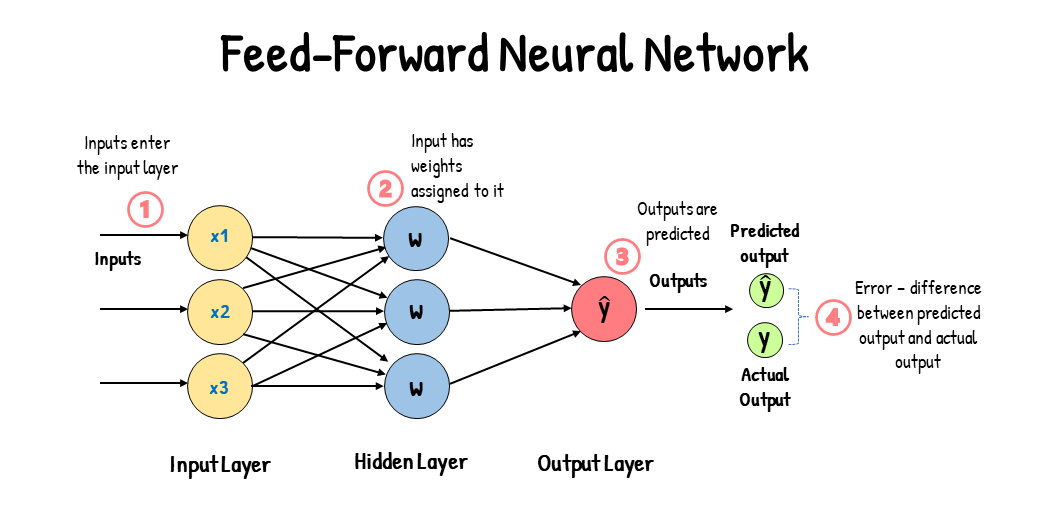
\includegraphics[width=9.0cm,keepaspectratio]{nn_working1}
\end{center}
\vspace{1mm}
\begin{takeawaybox}\footnotesize
Read it left to right: an input vector enters, each layer applies $\sigma(W\cdot+\mathbf{b})$, and a prediction leaves. \textbf{Every arrow is a multiplication by a number that will shortly be adjusted.}
\end{takeawaybox}
\end{frame}

%=============================================================================
\begin{frame}{A Classifier, on One Observation}
\begin{columns}[T]
\begin{column}{0.55\textwidth}
\small
The numbers on the next three frames come from the smallest honest version of 7.A1's digit classifier:
\medskip
\begin{itemize}\small\setlength{\itemsep}{1.2mm}
  \item \textbf{input} $x$ --- one feature of one image (in practice the flattened $784$-vector);
  \item \textbf{hidden and output} --- sigmoid units, so $\hat y\in[0,1]$ is the predicted probability that the image is a ``3'';
  \item \textbf{target} $t$ --- the true label, $1$ if it is a 3 and $0$ otherwise;
  \item \textbf{loss} $L$ --- squared error, for visibility; in practice cross-entropy.
\end{itemize}
\end{column}
\begin{column}{0.42\textwidth}
\begin{conceptbox}[title=\textbf{Why one observation?}]\small
Because the arithmetic is \textbf{identical} to training on millions: one forward pass, one loss, one backward pass, one update --- and then again.
\medskip
Everything that follows in this deck is about doing this faster, or stopping at the right time.
\end{conceptbox}
\end{column}
\end{columns}
\end{frame}

%=============================================================================
\begin{frame}{Forward, with Numbers}
\small
Input $x=1.0$, one sigmoid hidden unit, one sigmoid output unit, target $t=0$.
\vspace{-1mm}
\begin{columns}[T]
\begin{column}{0.50\textwidth}
\textbf{The network in full:}
\[ z_1=w_1x+b_1,\qquad h=\sigma(z_1) \]
\[ z_2=w_2h+b_2,\qquad \hat y=\sigma(z_2) \]
\[ L=\tfrac12(\hat y-t)^2 \]
{\footnotesize Parameters $w_1=0.5$, $b_1=0$, $w_2=2.0$, $b_2=0$.}
\smallskip

\textbf{With the numbers:}
\[ z_1=0.5\;\Rightarrow\;h=\sigma(0.5)\approx0.62 \]
\[ z_2=1.24\;\Rightarrow\;\hat y=\sigma(1.24)\approx0.78 \]
\[ L=\tfrac12(0.78)^2\approx0.30 \]
\end{column}
\begin{column}{0.47\textwidth}
\textbf{Reading it:}
\begin{itemize}\small\setlength{\itemsep}{1mm}
  \item $\sigma$ is a soft on/off switch: $z_1=0.5$ gives $h=0.62$, so the hidden unit is ``62\% on''.
  \item $\hat y=0.78$ is the predicted probability that this is a ``3''.
  \item The truth is $t=0$ --- it is \emph{not} a 3. The model is \textbf{confidently wrong}, and the loss is $0.30$.
  \item Learning means nudging $w_1,w_2$ so that $\hat y$ moves toward $t$. \textbf{How much each moves} is what backpropagation computes.
\end{itemize}
\end{column}
\end{columns}
\vspace{1mm}
\src{Ledger \texttt{backprop\_sigmoid.forward}. Code: \repo{tools/figures/s07_generate.py}{s07\_generate.py}, \texttt{run\_backprop\_sigmoid}; \repo{labs/L07_ML_and_Deep_Growth.ipynb}{L07} Part 3.}
\end{frame}

%=============================================================================
\begin{frame}{Backpropagation: Learning from a Mistake}
\begin{columns}[T]
\begin{column}{0.47\textwidth}
\small
\textbf{Goal.} $\partial L/\partial\theta$ for every parameter in the network.
\medskip

\textbf{Method.} The chain rule, applied backwards through the layers --- and \emph{organised}, so that each intermediate quantity is computed once and reused.
\medskip

\textbf{The loop:}
\begin{enumerate}\small\setlength{\itemsep}{0.8mm}
  \item forward: all activations, and the loss;
  \item backward: push the error signal from output to input;
  \item read off $\partial L/\partial W$, $\partial L/\partial\mathbf{b}$;
  \item update $\theta\leftarrow\theta-\eta\nabla_\theta L$.
\end{enumerate}
\end{column}
\begin{column}{0.50\textwidth}
\begin{center}
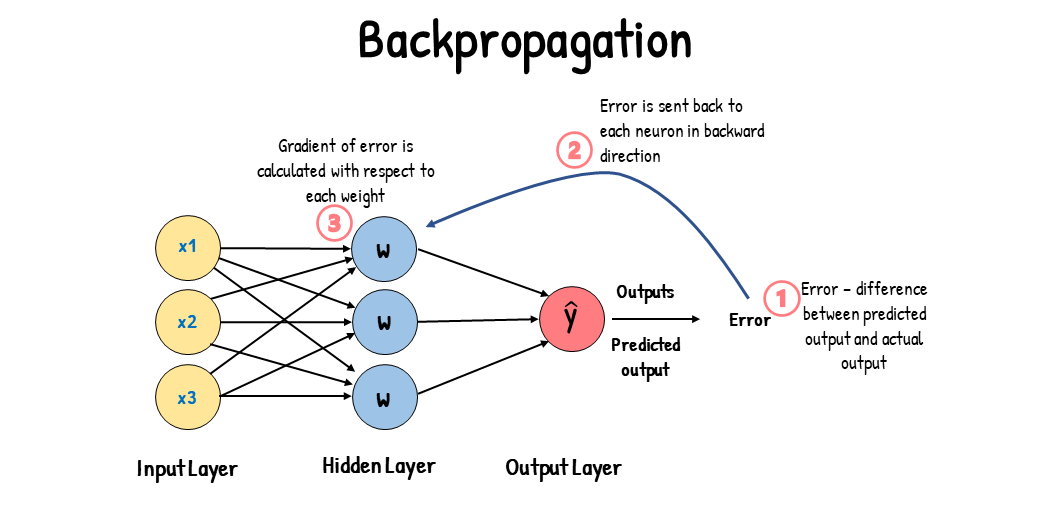
\includegraphics[width=7.0cm,keepaspectratio]{nn_working3}
\end{center}
\medskip
\begin{takeawaybox}\footnotesize
4.A4 already made the case: reverse mode gives a whole gradient for about the cost of \textbf{one} function evaluation, however many inputs there are. That is why this is possible at all.
\end{takeawaybox}
\end{column}
\end{columns}
\end{frame}

%=============================================================================
\begin{frame}{Backward, Part One: the Output Layer}
\footnotesize
Same example ($x=1.0$, $t=0$, $w_1=0.5$, $w_2=2.0$, $b_1=b_2=0$); forward gave $h\approx0.62$, $\hat y\approx0.78$, $L\approx0.30$.
\smallskip
\begin{columns}[T]
\begin{column}{0.58\textwidth}
\textbf{Chain the links $w_2\to z_2\to\hat y\to L$:}
\[
  \frac{\partial L}{\partial w_2}
  =\underbrace{\frac{\partial L}{\partial\hat y}}_{\hat y-t}\,
   \underbrace{\frac{\partial\hat y}{\partial z_2}}_{\hat y(1-\hat y)}\,
   \underbrace{\frac{\partial z_2}{\partial w_2}}_{h}
  =0.78\times0.17\times0.62\approx0.08
\]
The first two factors are worth a name, because they will be reused:
\[
  \delta_2\equiv\frac{\partial L}{\partial z_2}=(\hat y-t)\,\hat y(1-\hat y)\approx0.13 ,
\]
so $\partial L/\partial w_2=\delta_2 h$ and $\partial L/\partial b_2=\delta_2\approx0.13$.
\end{column}
\begin{column}{0.40\textwidth}
\centering
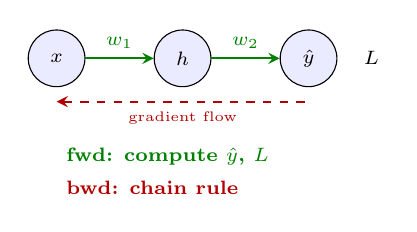
\begin{tikzpicture}[
    every node/.style={font=\scriptsize},
    layer/.style={circle, draw, minimum size=0.72cm, inner sep=0pt},
    fwd/.style={->, >=stealth, green!50!black, thick},
    bwd/.style={<-, >=stealth, red!70!black, thick, dashed}]
\node[layer, fill=blue!8] (x) at (0,0) {$x$};
\node[layer, fill=blue!8] (h) at (1.6,0) {$h$};
\node[layer, fill=blue!8] (y) at (3.2,0) {$\hat{y}$};
\node at (4.0,0) {$L$};
\draw[fwd] (x) -- (h) node[midway, above]{$w_1$};
\draw[fwd] (h) -- (y) node[midway, above]{$w_2$};
\draw[bwd] (0,-0.55) -- node[midway, below, font=\tiny]{gradient flow} (3.2,-0.55);
\node[green!50!black, font=\scriptsize\bfseries, anchor=west] at (0,-1.25) {fwd: compute $\hat y$, $L$};
\node[red!70!black, font=\scriptsize\bfseries, anchor=west] at (0,-1.65) {bwd: chain rule};
\end{tikzpicture}
\smallskip

\raggedright\textbf{Read the sign.} $\partial L/\partial w_2>0$, so raising $w_2$ would \emph{raise} the loss --- descent lowers it. The output overshot $t=0$.
\end{column}
\end{columns}
\vspace{1mm}
\src{Ledger \texttt{backprop\_sigmoid.backward}. Code: \repo{tools/figures/s07_generate.py}{s07\_generate.py}; \repo{labs/L07_ML_and_Deep_Growth.ipynb}{L07} Part 3.}
\end{frame}

%=============================================================================
\begin{frame}{Backward, Part Two: One Layer Further, and the Update}
\begin{columns}[T]
\begin{column}{0.56\textwidth}
\small
Carry $\delta_2\approx0.13$ back through $w_2$, then through the hidden activation:
\[
  \frac{\partial L}{\partial h}=\delta_2 w_2\approx0.26,\qquad
  \frac{\partial h}{\partial z_1}=h(1-h)\approx0.24 ,
\]
\[
  \delta_1\equiv\frac{\partial L}{\partial z_1}=\frac{\partial L}{\partial h}\cdot\frac{\partial h}{\partial z_1}\approx0.06 ,
\]
and finally $\partial L/\partial w_1=\delta_1 x\approx0.06$.
\medskip

\textbf{The update.} Step against the gradient at \textbf{learning rate} $\eta=0.1$ --- the one free choice in the algorithm, $w\leftarrow w-\eta\,\partial L/\partial w$:
\[
  w_2\leftarrow2.0-0.1(0.0839)=1.992 ,
\]
and likewise $w_1\leftarrow0.494$.
\end{column}
\begin{column}{0.41\textwidth}
\begin{takeawaybox}[title=\textbf{That is the whole algorithm}]\small
Exactly what \texttt{loss.backward()} and one optimizer step do in 3.B3's five-line loop --- at millions of parameters, and not otherwise different.
\medskip
And look at the two factors $\hat y(1-\hat y)$ and $h(1-h)$: neither exceeds $\mathbf{0.25}$. Every extra sigmoid layer multiplies the signal by one more of them --- 7.A2's vanishing gradient, seen from the other end.
\end{takeawaybox}
\end{column}
\end{columns}
\vspace{1mm}
\src{Ledger \texttt{backprop\_sigmoid}, checked against \texttt{autograd}. Code: \repo{tools/figures/s07_generate.py}{s07\_generate.py}; \repo{labs/L07_ML_and_Deep_Growth.ipynb}{L07} Part 3.}
\end{frame}

%=============================================================================
\begin{frame}{The Same Thing with ReLU, in Four Parameters}
\begin{columns}[T]
\begin{column}{0.55\textwidth}
\small
$x=2$, $y=3$, one ReLU hidden unit, $L=(\hat y-y)^2$, and $(w_1,b_1,v,c)=(0.5,-0.1,1.2,0.3)$.
\medskip

\textbf{Forward.} $z=0.9$, $h=0.9$, $\hat y=1.38$, $L=2.6244$.
\medskip

\textbf{Backward.}
\[
  \frac{\partial L}{\partial\hat y}=2(\hat y-y)=-3.24,\quad
  \frac{\partial L}{\partial v}=-2.916,
\]
\[
  \frac{\partial L}{\partial h}=-3.888,\quad
  \frac{\partial L}{\partial z}=-3.888,\quad
  \frac{\partial L}{\partial w_1}=-7.776 .
\]
\textbf{Update} at $\eta=0.01$: $w_1^{\text{new}}=0.5778$.
\end{column}
\begin{column}{0.42\textwidth}
\begin{conceptbox}[title=\textbf{What changed, and what did not}]\small
The recipe is identical. Only $\partial h/\partial z$ differs: for ReLU it is $\mathbf{1}$ on the active side and $\mathbf{0}$ on the other.
\medskip
\textbf{No shrinkage factor.} That single fact is most of why ReLU replaced the sigmoid in hidden layers.
\end{conceptbox}
\medskip
\begin{examplebox}\footnotesize
And the zero is real: a unit whose input is negative for every sample receives no gradient at all and never recovers. That is the ``dying ReLU'', and it is why 7.A2 listed Leaky ReLU.
\end{examplebox}
\end{column}
\end{columns}
\vspace{1mm}
\src{Feng \& Miao, \emph{AI for Economists}, ch.~9 \S9.3.2. Ledger \texttt{backprop\_worked}; every figure reproduced by running it, agreeing with \texttt{autograd} to machine precision. Code: \repo{tools/figures/s07_generate.py}{s07\_generate.py}, \texttt{run\_backprop\_worked}.}
\end{frame}

%=============================================================================
\begin{frame}{The Recursion, in General}
\begin{columns}[T]
\begin{column}{0.54\textwidth}
\small
The forward pass ends in an affine output and a loss, and the error signal $\boldsymbol\delta^{(\ell)}=\partial\mathcal{L}/\partial\mathbf{z}^{(\ell)}$ \textbf{starts there}:
\[
  \hat{\mathbf y}=W_{L+1}\mathbf{h}^{(L)}+\mathbf{b}_{L+1},\quad
  \mathcal{L}=\tfrac12\lVert\hat{\mathbf y}-\mathbf y\rVert^{2},\quad
  \boldsymbol\delta^{(L+1)}=\hat{\mathbf y}-\mathbf y .
\]
The rest is two lines:
\[
  \boldsymbol\delta^{(\ell)}=\bigl(W_{\ell+1}^{\top}\boldsymbol\delta^{(\ell+1)}\bigr)\odot\sigma'\bigl(\mathbf{z}^{(\ell)}\bigr),
\]
\[
  \frac{\partial\mathcal{L}}{\partial W_\ell}=\boldsymbol\delta^{(\ell)}\bigl(\mathbf{h}^{(\ell-1)}\bigr)^{\top},
  \qquad
  \frac{\partial\mathcal{L}}{\partial\mathbf{b}_\ell}=\boldsymbol\delta^{(\ell)} .
\]
\medskip

Read the first: transpose the \emph{same} weight matrix used going forward, apply it to the signal above, multiply pointwise by the local slope. Read the second: the gradient at a weight is the signal on its output side times the activation on its input side.
\end{column}
\begin{column}{0.43\textwidth}
\begin{takeawaybox}\small
\textbf{Two facts follow immediately.}
\medskip
\textbf{(1)} $\sigma'$ multiplies at every layer, so the activation choice controls whether the signal survives depth.
\medskip
\textbf{(2)} $\mathbf{h}^{(\ell-1)}$ is needed on the way back, so the \textbf{forward activations must be stored} --- the memory cost of training, and why batch size is limited by the card.
\end{takeawaybox}
\end{column}
\end{columns}
\vspace{1mm}
\src{Feng \& Miao, \emph{AI for Economists}, ch.~9, eqs.~(9.20)--(9.21).}
\end{frame}

%=============================================================================
\begin{frame}{Backpropagation Is the Adjoint Method}
\begin{columns}[T]
\begin{column}{0.54\textwidth}
\small
$\boldsymbol\delta^{(\ell)}$ is the derivative of the objective with respect to an \emph{intermediate quantity} --- how much the loss would change if $\mathbf{z}^{(\ell)}$ were perturbed and everything downstream re-optimised.
\medskip

\textbf{That is a shadow price.} It is the multiplier on the constraint ``$\mathbf{z}^{(\ell)}$ is what the previous layer produced'', and the backward recursion is exactly the costate equation run from the terminal condition backwards.
\medskip

The technique has a name in optimal control: the \textbf{adjoint method}. Backpropagation is the adjoint method on a discrete computation graph.
\end{column}
\begin{column}{0.43\textwidth}
\begin{conceptbox}[title=\textbf{Why this is worth a slide}]\small
You already know how to read a multiplier. $\delta$ large means that layer's output matters a great deal at the current parameters; $\delta\approx0$ means it does not, and no amount of adjusting the weights below it will help.
\medskip
A \emph{diagnosis}, not a metaphor: printing per-layer gradient norms is standard practice for exactly this reason.
\end{conceptbox}
\smallskip
\begin{examplebox}\footnotesize
1.B1's Lagrangian and 5.A1's implicit-function argument are the same mathematics, met a third time.
\end{examplebox}
\end{column}
\end{columns}
\vspace{1mm}
\src{Feng \& Miao, \emph{AI for Economists}, ch.~9 \S9.3.2, the ``shadow price'' discussion.}
\end{frame}

%=============================================================================
\begin{frame}{One Graph, Two Traversals --- and What It Costs}
\begin{columns}[T]
\begin{column}{0.53\textwidth}
\small
The forward pass and the backward pass are two traversals of \textbf{one} object: the computation graph, whose nodes are tensors and whose edges are operations. 3.B3 built it; this is what it is for.
\medskip

The cost follows from the structure. With $P$ parameters, one sample:
\begin{itemize}\small\setlength{\itemsep}{1mm}
  \item forward $\approx 2P$ floating-point operations (a multiply and an add per weight);
  \item backward $\approx 4P$ --- the signal to the layer below, \emph{and} the gradient at the weight;
  \item total $\approx 6P$ per sample per pass.
\end{itemize}
\[
  \text{FLOPs}\;\approx\;6\,P\,n\,E
\]
for $n$ samples and $E$ epochs.
\end{column}
\begin{column}{0.44\textwidth}
\begin{takeawaybox}[title=\textbf{Use it as a budget}]\small
$P=10^{5}$, $n=5\times10^{4}$, $E=100$ needs about $3\times10^{12}$ FLOPs --- seconds of real arithmetic. \textbf{A tabular macro network is not a big computation:} dozens of configurations are affordable without a GPU.
\end{takeawaybox}
\smallskip
{\footnotesize A chip's advertised \textbf{peak} FLOPS is never achieved --- measured utilisation is $21.3\%$ for GPT-3, $46.2\%$ for PaLM-540B. A runtime worked out from peak is optimistic: \textbf{multiply it by two to four}.}
\end{column}
\end{columns}
\vspace{1mm}
\src{Feng \& Miao, \emph{AI for Economists}, ch.~9 \S9.3.4; the $6N$ convention follows Kaplan et al.\ (2020), the utilisation figures Chowdhery et al.\ (2023).}
\end{frame}

%=============================================================================
\begin{frame}{Gradient Descent: the Engine}
\begin{columns}[T]
\begin{column}{0.54\textwidth}
\small
One update rule covers everything in this deck:
\[
  \theta_{n+1}\;\leftarrow\;\theta_n-\lambda_n\,g(b_n;\theta_n),
\]
where $g$ is the gradient computed on a batch $b_n$ of size $n$:
\begin{itemize}\small\setlength{\itemsep}{1mm}
  \item $n=1$: \textbf{stochastic} gradient descent --- one draw per step;
  \item $n=N$: \textbf{full} gradient descent --- the whole sample per step;
  \item $1<n<N$: \textbf{mini-batch} --- what everyone actually does.
\end{itemize}
\medskip
\[
  \frac{d\mathcal{L}(\theta)}{d\theta}\;\approx\;\frac{1}{n}\sum_{i=1}^{n}\frac{d\mathcal{L}(\theta;b_i)}{d\theta}
\]
\end{column}
\begin{column}{0.43\textwidth}
\begin{conceptbox}[title=\textbf{The algorithm, entire}]\small
\begin{enumerate}\small\setlength{\itemsep}{0.7mm}
  \item initialise $\theta$ at random;
  \item draw a mini-batch, form $g(b_n;\theta_n)$;
  \item pick $\lambda_n>0$ and step;
  \item repeat.
\end{enumerate}
\end{conceptbox}
\medskip
\begin{takeawaybox}\footnotesize
\textbf{This is 4.A3's $M$-sum.} There the sampled gradient was introduced on a two-term objective; here the terms are observations, or sampled states. The object is the same.
\end{takeawaybox}
\end{column}
\end{columns}
\end{frame}

%=============================================================================
\begin{frame}{Descent, Drawn}
\begin{center}
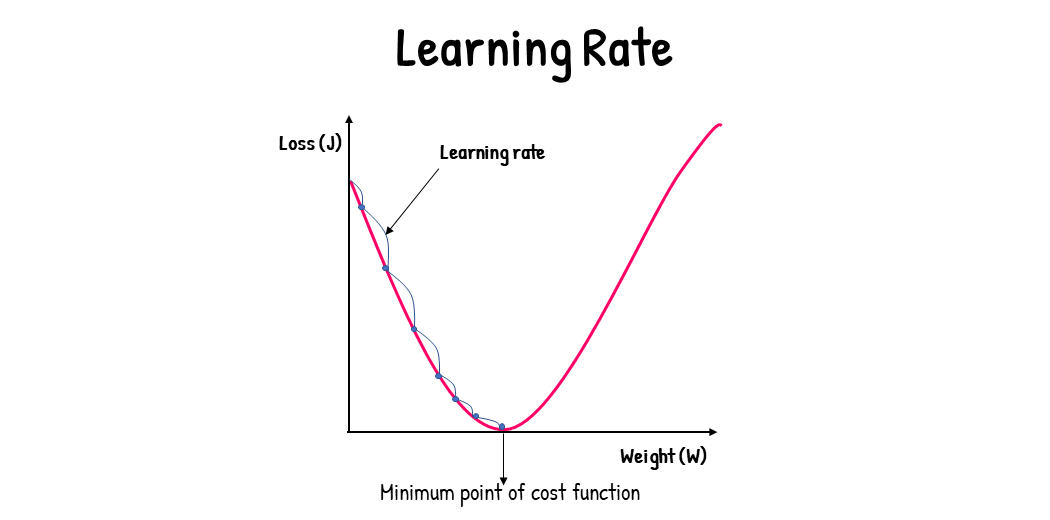
\includegraphics[width=8.6cm,keepaspectratio]{nn_working6}
\end{center}
\vspace{1mm}
\begin{takeawaybox}\footnotesize
The picture is 4.A3's, redrawn: step against the gradient, with the step length the only real decision. What the picture cannot show is that this surface has $10^{5}$ axes, which is the subject of the next two frames.
\end{takeawaybox}
\end{frame}

%=============================================================================
\begin{frame}{Why Not Newton --- 4.A3 Already Answered This}
\begin{columns}[T]
\begin{column}{0.48\textwidth}
\small
Session 4 spent a block on second-order methods and closed with the frame that settles this one. A Hessian for $N$ parameters has $N^{2}$ entries, and \textbf{numbers that must be stored} grow accordingly:
\medskip

\begin{center}\footnotesize
\begin{tabularx}{\linewidth}{@{}>{\raggedright\arraybackslash}p{1.35cm} >{\raggedleft\arraybackslash}X >{\raggedleft\arraybackslash}X >{\raggedleft\arraybackslash}X@{}}
\toprule
$N$ & \textbf{Newton} & \textbf{L-BFGS} & \textbf{CG} \\
\midrule
$10^{2}$ & $10^{4}$ & $2{,}000$ & $300$ \\
$10^{4}$ & $10^{8}$ & $2\times10^{5}$ & $3\times10^{4}$ \\
$10^{6}$ & $\mathbf{10^{12}}$ & $2\times10^{7}$ & $3\times10^{6}$ \\
\bottomrule
\end{tabularx}
\end{center}
\medskip
$N=10^{6}$ is the parameter count of a \emph{small} network.
\end{column}
\begin{column}{0.49\textwidth}
\begin{cautionbox}[title=\textbf{The frame this cites}]\small
4.A3 put it plainly: $10^{12}$ Hessian entries is why \textbf{nobody trains a network with Newton's method}, and why Session 7's optimizer is a first-order one.
\medskip
That promise is now kept. Everything from here on uses gradients only.
\end{cautionbox}
\medskip
\begin{examplebox}\footnotesize
Note that even L-BFGS with ten stored pairs needs $2\times10^{7}$ numbers at $N=10^{6}$ --- affordable, and still not what is used, for the reason on the next frame.
\end{examplebox}
\end{column}
\end{columns}
\vspace{1mm}
\src{Ledger \texttt{optimizer\_memory} from \texttt{s04\_numbers.json} --- cited, not recomputed. Code: \repo{tools/figures/s04_generate.py}{s04\_generate.py}.}
\end{frame}

%=============================================================================
\begin{frame}{And Why Not Conjugate Gradient Either}
\begin{columns}[T]
\begin{column}{0.53\textwidth}
\small
4.A3's other result was that conjugate gradient is \textbf{exact in at most $N$ steps} on an $N$-dimensional quadratic, storing only a handful of vectors. On the two-dimensional example it reached the optimum from $(2,2)$ in \textbf{two} steps, with the intermediate point $(0.889,-0.222)$.
\medskip

So why is it not the method here? Because both CG and L-BFGS need a gradient that is \textbf{the same function every time they are asked}. Line searches and conjugacy corrections assume a fixed objective.
\medskip

A mini-batch gradient is a \textbf{different} function at every step. The conjugacy that CG constructs is destroyed by the noise before it can be used.
\end{column}
\begin{column}{0.44\textwidth}
\begin{takeawaybox}[title=\textbf{The trade, stated once}]\small
Second-order and conjugate methods buy \textbf{accuracy per step}, and pay in memory and in the requirement of an exact gradient.
\medskip
Training a network wants the opposite: \textbf{very many cheap, noisy steps}. The noise is not merely tolerated --- the next frames argue it helps.
\end{takeawaybox}
\medskip
\begin{examplebox}\footnotesize
The exception proves it: \emph{full-batch} L-BFGS is a perfectly sensible choice for a small collocation problem, and is what a projection solver uses.
\end{examplebox}
\end{column}
\end{columns}
\vspace{1mm}
\src{Ledger \texttt{cg\_steps} from \texttt{s04\_numbers.json} --- cited, not recomputed. Code: \repo{tools/figures/s04_generate.py}{s04\_generate.py}.}
\end{frame}

%=============================================================================
\begin{frame}{Why a Sampled Gradient Still Gets There}
\begin{columns}[T]
\begin{column}{0.52\textwidth}
\small
\textbf{Every loss here is a sum over terms,} $\mathcal{L}=\frac1N\sum_i\ell_i$ --- one per observation, in Block B one per sampled state --- and \textbf{SGD differentiates one term at a time.} 4.A3 ran that on the smallest case: two terms, $\ell_1=\tfrac12x^2$, $\ell_2=y^2$, from $(2,2)$ at step size $\lambda=0.5$, full gradient $(2,4)$. \textbf{``Drawn'' is the term the step used:}
\medskip

\begin{center}\footnotesize
\begin{tabularx}{\linewidth}{@{}>{\raggedright\arraybackslash}p{1.6cm} >{\raggedright\arraybackslash}p{1.0cm} >{\raggedright\arraybackslash}X@{}}
\toprule
$\theta$ & \textbf{drawn} & \textbf{next} \\
\midrule
$(2,2)$ & $\ell_2$ & $(2,0)$ \\
$(2,0)$ & $\ell_1$ & $(1,0)$ \\
$(1,0)$ & $\ell_1$ & $(0.5,0)$ \\
$(0.5,0)$ & $\ell_2$ & $(0.5,0)$ \\
$(0.5,0)$ & $\ell_1$ & $(0.25,0)$ \\
\bottomrule
\end{tabularx}
\end{center}
\vspace{-2mm}
{\footnotesize \textbf{A coordinate whose term was not drawn does not move}; row four draws $\ell_2$ at $y=0$ and does nothing. The path is not monotone, and is not meant to be.}
\end{column}
\begin{column}{0.45\textwidth}
\begin{cautionbox}[title=\textbf{And why it still works}]\footnotesize
4.A3 measured how the noise scales with the \textbf{number of parameters} $P$ --- not the sample size. Its norm grows like $\sqrt P$: $1$, $10$, $100$, $1{,}000$ at $P=1,10^{2},10^{4},10^{6}$, while the \emph{useful} component grows with the full gradient. The ratio degrades slowly enough that very many cheap steps beat few exact ones.
\end{cautionbox}
\medskip
{\footnotesize \textbf{Mini-batches are that sum}, and the schedule below is Robbins--Monro. Nothing in this optimizer is new; only its scale is.}
\end{column}
\end{columns}
\vspace{1mm}
\src{Ledger \texttt{sgd\_trajectory}, \texttt{sgd\_dimension} from \texttt{s04\_numbers.json} --- cited, not recomputed. Code: \repo{tools/figures/s04_generate.py}{s04\_generate.py}.}
\end{frame}

%=============================================================================
\begin{frame}{Batch, Stochastic, Mini-Batch}
\begin{columns}[T]
\begin{column}{0.33\textwidth}
\begin{center}
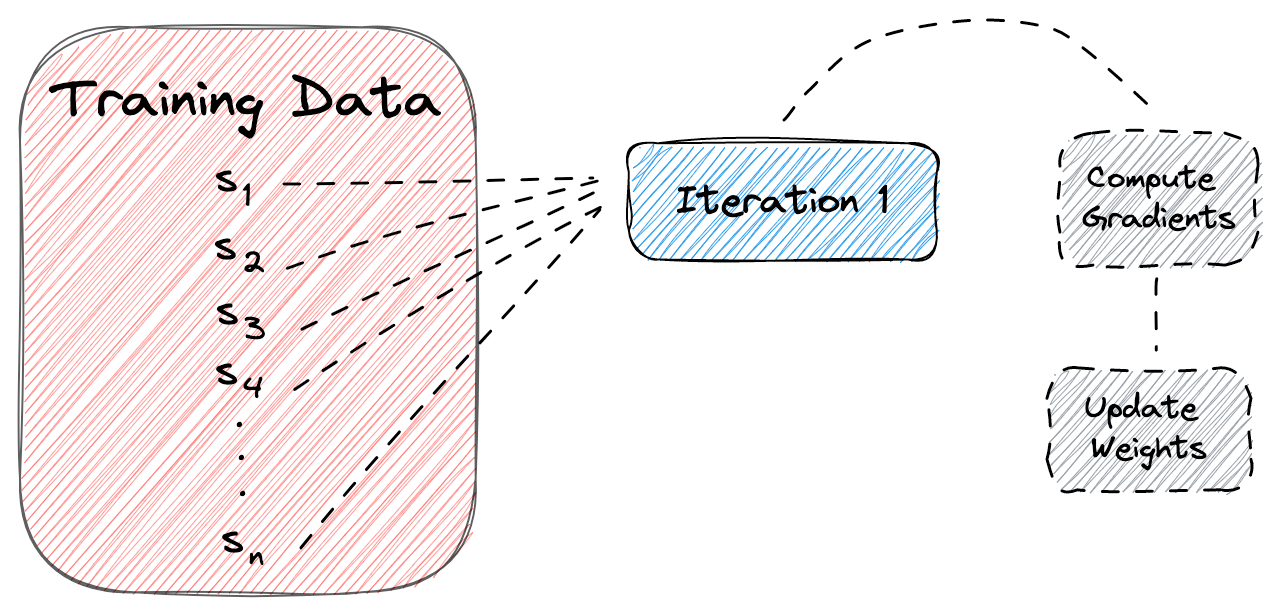
\includegraphics[width=\linewidth,height=2.5cm,keepaspectratio]{batch_1}
\end{center}
{\scriptsize \textbf{Batch.} A smooth path, and every step expensive --- it uses all the data.}
\end{column}
\begin{column}{0.33\textwidth}
\begin{center}
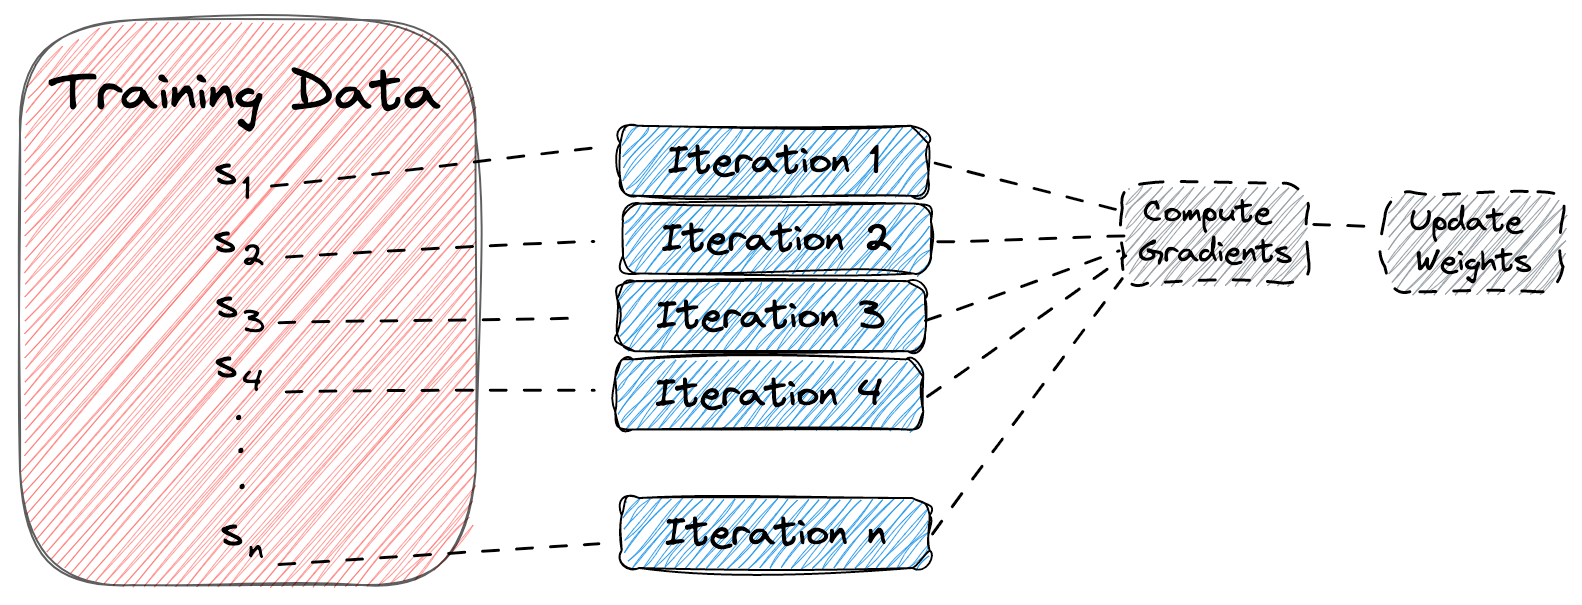
\includegraphics[width=\linewidth,height=2.5cm,keepaspectratio]{batch_2}
\end{center}
{\scriptsize \textbf{Stochastic.} A noisy, high-variance path; each step is cheap, and the noise can leave a poor minimum.}
\end{column}
\begin{column}{0.33\textwidth}
\begin{center}
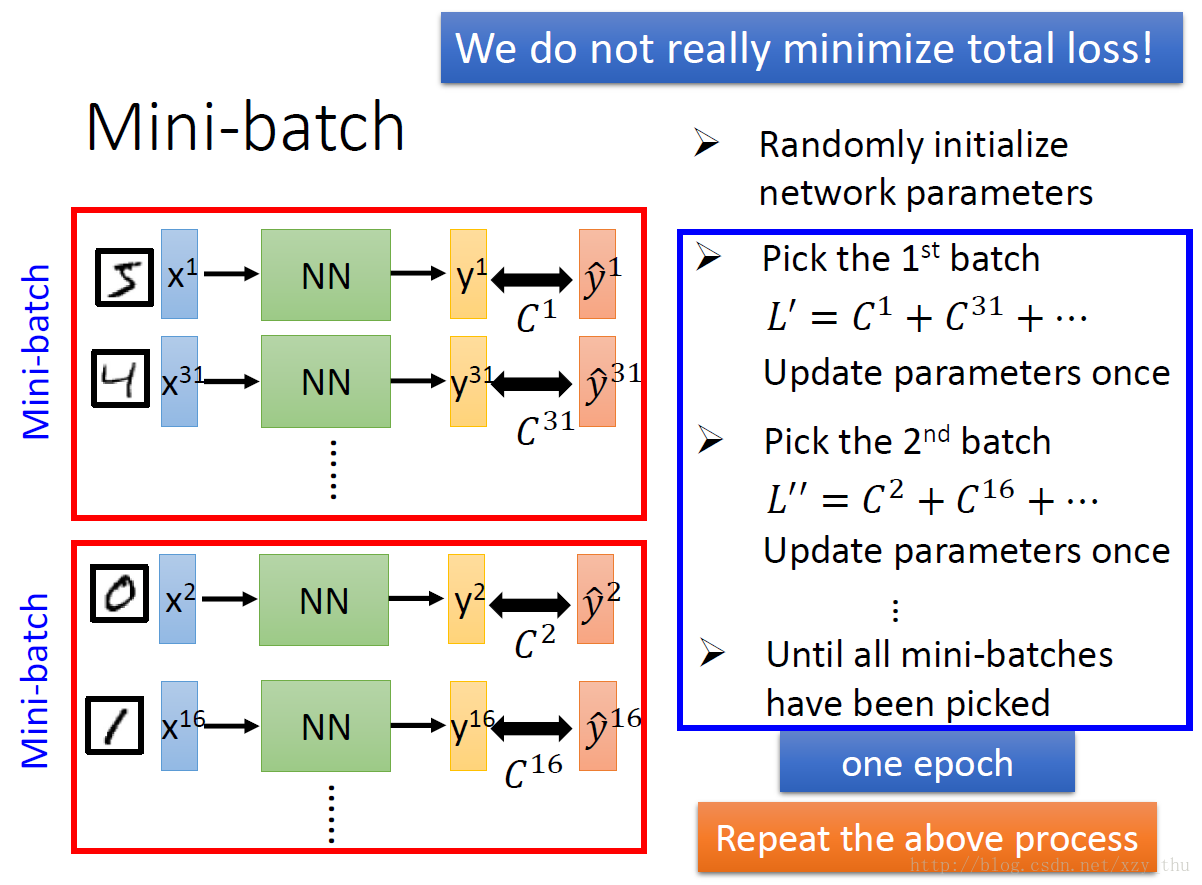
\includegraphics[width=\linewidth,height=2.5cm,keepaspectratio]{minibatch}
\end{center}
{\scriptsize \textbf{Mini-batch.} Parallelisable like the first, averaged like the second. The practical standard.}
\end{column}
\end{columns}
\vspace{1mm}
\begin{takeawaybox}\footnotesize
The three pictures are the same descent with three answers to one question: \textbf{how many terms of the sum do you look at before you move?}
\end{takeawaybox}
\end{frame}

%=============================================================================
\begin{frame}{Why Mini-Batch? Four Reasons}
\begin{columns}[T]
\begin{column}{0.55\textwidth}
\small
\begin{enumerate}\small\setlength{\itemsep}{1.4mm}
  \item \textbf{Computational efficiency.} Far more updates per pass over the data than full gradient descent, and so faster convergence in wall-clock time.
  \item \textbf{Memory.} The activations of a full dataset do not fit on a card --- and the previous frames showed they must be stored.
  \item \textbf{Implicit regularisation.} The noise in the gradient estimate helps the iterate leave saddle points and shallow minima. It is doing statistical work, not just saving time.
  \item \textbf{Parallelisation.} A batch is a matrix multiplication, which is what the hardware is for.
\end{enumerate}
\end{column}
\begin{column}{0.42\textwidth}
\begin{takeawaybox}[title=\textbf{The econometric analogue}]\small
Mini-batch descent is sampling-based estimation: trade exactness for speed --- and find that the noise is \textbf{helpful}, not merely tolerable.
\end{takeawaybox}
\medskip
\begin{examplebox}\footnotesize
In 7.B1 there is no dataset, so ``batch'' means \textbf{a fresh draw of states} each step. Nothing is ever reused, and reason (3) is doing most of the work.
\end{examplebox}
\end{column}
\end{columns}
\end{frame}

%=============================================================================
\begin{frame}{Convergence: What Is Actually Guaranteed}
\begin{columns}[T]
\begin{column}{0.55\textwidth}
\small
Under a Lipschitz gradient and bounded gradient-noise variance, if the step sizes satisfy
\[
  \sum_{n=1}^{\infty}\lambda_n=\infty
  \qquad\text{and}\qquad
  \sum_{n=1}^{\infty}\lambda_n^{2}<\infty ,
\]
then the weighted average of expected squared gradients vanishes:
\[
  \mathbb{E}\!\left[\frac{1}{\Delta_N}\sum_{n=1}^{N}\lambda_n\lVert\nabla F(\theta_n)\rVert^{2}\right]\;\longrightarrow\;0,
  \qquad \Delta_N=\sum_{n=1}^{N}\lambda_n .
\]
\medskip

In words: with the step size shrinking at the right rate, stochastic gradient descent settles at a \textbf{stationary point}.
\end{column}
\begin{column}{0.42\textwidth}
\begin{cautionbox}[title=\textbf{Read the statement carefully}]\small
It promises a \emph{stationary point} --- not a global minimum, not even a local one, and it says nothing about how long.
\medskip
Compare 3.A2's value-function iteration, where the contraction gave a \textbf{unique} fixed point and a computable error bound. \textbf{That is what is being given up}, and it is the honest price of the learned basis.
\end{cautionbox}
\end{column}
\end{columns}
\vspace{1mm}
\src{Bottou, Curtis \& Nocedal (2018), \emph{Optimization Methods for Large-Scale Machine Learning}.}
\end{frame}

%=============================================================================
\begin{frame}{The Robbins--Monro Conditions, Read as Economics}
\small
These are the \textbf{Robbins--Monro} conditions (1951), the foundation of \emph{stochastic approximation} --- driving a noisy signal to its root. That is exactly what descent on a mini-batch gradient is.
\vspace{-1mm}
\begin{columns}[T]
\begin{column}{0.49\textwidth}
\begin{conceptbox}\small
\textbf{$\sum\lambda_n=\infty$ --- ``go the distance.''}
The steps must sum to infinity so the iterate can travel \emph{any} distance, however far the start. Decay too fast and the total path length is finite: training \textbf{stalls short}.
\end{conceptbox}
\end{column}
\begin{column}{0.49\textwidth}
\begin{conceptbox}\small
\textbf{$\sum\lambda_n^{2}<\infty$ --- ``kill the noise.''}
The squared steps must be summable so accumulated gradient noise stays finite and dies. This forces $\lambda_n\to0$ fast enough that late steps stop bouncing and the iterate \textbf{settles}.
\end{conceptbox}
\end{column}
\end{columns}
\medskip
\begin{itemize}\small\setlength{\itemsep}{1mm}
  \item \textbf{Concretely:} $\lambda_n=1/n$ satisfies both. $\lambda_n=1/\sqrt n$ satisfies the first and fails the second --- too noisy. A \textbf{constant} $\lambda$ also fails the second, and SGD then bounces forever in a ball around the optimum, which is exploration, not convergence.
  \item \textbf{4.A3 named this already.} The learning-rate schedule is not a hyperparameter with a folklore value; it is the condition under which the sampled-gradient recursion has a limit at all.
\end{itemize}
\vspace{1mm}
\src{Robbins \& Monro (1951). The same recursion underlies recursive and online estimation in econometrics.}
\end{frame}

%=============================================================================
\begin{frame}{Adaptive Step Sizes: RProp $\to$ RMSProp $\to$ Adam}
\begin{columns}[T]
\begin{column}{0.58\textwidth}
\small
\textbf{RProp} (Riedmiller \& Braun, 1993) sizes each parameter's step from the \textbf{sign} of its gradient alone. Robust --- but the signs are too noisy once batches are sampled.
\medskip

\textbf{RMSProp} (Hinton, 2012) adapts that to mini-batches: give each parameter its own step by dividing by a running average of \emph{squared} gradients,
\[
  r_{k+1}\leftarrow\rho\,r_k+(1-\rho)\,g_k\odot g_k,
\]
\[
  \Delta\theta_{k+1}=-\frac{\lambda}{\sqrt{\delta+r_{k+1}}}\odot g_k ,
\]
damping steep directions and amplifying flat ones.
\medskip

\textbf{Adam} (Kingma \& Ba, 2015) is momentum \emph{and} RMSProp: running averages of the gradient and of its square, with decay rates $\rho_1,\rho_2$ (defaults $0.9$, $0.999$).
\end{column}
\begin{column}{0.39\textwidth}
\begin{takeawaybox}[title=\textbf{What Adam is, in one line}]\small
\textbf{Adam is stochastic gradient descent with a per-parameter step size.}
\medskip
It is still first-order. It never forms, stores or inverts a Hessian --- which is precisely the constraint the memory-wall frame imposed.
\end{takeawaybox}
\medskip
\begin{examplebox}\footnotesize
The economist's reading of momentum: an exponentially weighted average of past gradients is \textbf{adaptive expectations} over the descent direction.
\end{examplebox}
\end{column}
\end{columns}
\vspace{1mm}
\src{Kingma \& Ba (2015); Hinton (2012); Riedmiller \& Braun (1993). Adam was the default choice from 2015 until roughly 2022.}
\end{frame}

%=============================================================================
\begin{frame}{Beyond Adam}
\begin{columns}[T]
\begin{column}{0.54\textwidth}
\small
\begin{itemize}\small\setlength{\itemsep}{1.3mm}
  \item \textbf{AdamW} (Loshchilov \& Hutter, 2019) --- decoupled weight decay; the de-facto default.
  \item \textbf{Lion} (Chen et al., 2023) --- a sign-based update, lower memory than Adam, competitive at large scale.
  \item \textbf{Sophia} (Liu et al., 2023) --- a cheap second-order method using a \emph{diagonal} Hessian estimate. Note what makes it affordable: the diagonal is $N$ numbers, not $N^{2}$.
  \item \textbf{Schedule-free} methods (Defazio et al., 2024) --- drop the learning-rate schedule; the optimizer self-regulates.
\end{itemize}
\end{column}
\begin{column}{0.43\textwidth}
\begin{takeawaybox}[title=\textbf{Course default}]\small
\texttt{torch.optim.AdamW(lr=1e-3,}\\
\texttt{\ \ weight\_decay=1e-2)}
\medskip
for every lab in this course, varied only where a slide says so.
\end{takeawaybox}
\medskip
\begin{conceptbox}\footnotesize
\textbf{The economist's take:} choosing an optimizer is choosing a numerical solver --- it depends on the geometry of the problem. At the $10^{3}$--$10^{6}$ parameter scale of macro networks, AdamW is the safe answer.
\end{conceptbox}
\end{column}
\end{columns}
\end{frame}

%=============================================================================
\begin{frame}{Loss I: Squared Error Is OLS}
\begin{columns}[T]
\begin{column}{0.55\textwidth}
\small
For a continuous target,
\[
  \mathcal{L}_{\text{MSE}}=\frac{1}{N}\sum_{i=1}^{N}(\hat y_i-y_i)^{2},
\]
the average squared gap, with big misses penalised quadratically.
\medskip

\textbf{Why this form and not another?} Minimising it is \textbf{exactly maximum likelihood under Gaussian errors}; for a linear model it \emph{is} OLS. The loss is not a convention --- it encodes an assumption about the noise.
\medskip

Change the noise model and the loss changes with it: Poisson for counts, pinball for quantiles.
\end{column}
\begin{column}{0.42\textwidth}
\begin{takeawaybox}[title=\textbf{Where this lands}]\small
GDP growth, yields, prices --- and, in 7.B1, \textbf{Euler-equation residuals}.
\medskip
There the ``target'' is zero and the ``prediction'' is the residual, so minimising MSE is asking the equilibrium condition to hold. \textbf{No data enters.}
\end{takeawaybox}
\medskip
\begin{examplebox}\footnotesize
And 5.B5 already told you what that is: a \emph{least-squares weighted residual}. The loss function of a neural solver has a name in Session 5.
\end{examplebox}
\end{column}
\end{columns}
\end{frame}

%=============================================================================
\begin{frame}{Loss II: Cross-Entropy Is McFadden}
\footnotesize
A classifier chooses among $K$ classes; the network emits a raw score $z_k$ per class and \textbf{softmax} turns the scores into probabilities:
\[
  \hat y_k=\frac{e^{z_k}}{\sum_{j}e^{z_j}},\qquad \sum_k\hat y_k=1 .
\]
The label is \textbf{one-hot}: $y$ has a single $1$ at the true class. A true ``3'' is $y=(0,0,0,1,0,\dots,0)$.
\smallskip
\begin{columns}[T]
\begin{column}{0.53\textwidth}
\textbf{Cross-entropy:}
\[
  \mathcal{L}_{\text{CE}}=-\sum_k y_k\log\hat y_k=-\log\hat y_{k^{\star}} .
\]
Every term vanishes but the true one, so CE is \textbf{the negative log-probability assigned to the correct answer}. Minimising it maximises that probability: $\hat y_{k^{\star}}=0.99$ gives $0.01$; $\hat y_{k^{\star}}=0.1$ gives $2.3$. Confident and right costs nothing; confident and wrong is unbounded.
\end{column}
\begin{column}{0.45\textwidth}
\begin{takeawaybox}\footnotesize
\textbf{This is McFadden (1973).} Softmax is the logit choice probability, the one-hot $y$ is the observed choice, and minimising cross-entropy is maximising the multinomial-logit log-likelihood.
\medskip
\textbf{Classification is discrete choice.} You have estimated this model; you have not called it a loss function before.
\end{takeawaybox}
\end{column}
\end{columns}
\vspace{1mm}
\src{McFadden (1973), ``Conditional Logit Analysis of Qualitative Choice Behavior''. The binary toy above is the $K=2$ case.}
\end{frame}

%=============================================================================
\begin{frame}{Terminology, and the Arithmetic Behind It}
\begin{columns}[T]
\begin{column}{0.54\textwidth}
\small
\begin{itemize}\small\setlength{\itemsep}{1.2mm}
  \item \textbf{Epoch} --- one complete pass through the training data.
  \item \textbf{Mini-batch} --- the subset used for one update.
  \item \textbf{Iteration} --- one parameter update, that is, one mini-batch.
  \item \textbf{Automatic differentiation} --- the exact-gradient machinery behind \texttt{loss.backward()} (3.B3, 4.A4).
  \item \textbf{Episode} --- a reinforcement-learning term: one path from an initial to a terminal state. It is a simulated life cycle, and it belongs to S8.
\end{itemize}
\end{column}
\begin{column}{0.43\textwidth}
\begin{conceptbox}[title=\textbf{Do the arithmetic once}]\small
With $n=50{,}000$ and batch $256$, one epoch is 156 iterations. At $100$ epochs that is about 15{,}600 updates.
\medskip
\textbf{``Epochs'' is not the unit that matters --- updates is.} The same 100 epochs on $n=2{,}000$ is only about 600 updates, which is why a small sample needs far more epochs to reach the same place.
\end{conceptbox}
\end{column}
\end{columns}
\vspace{1mm}
\src{Step counts from ledger \texttt{epoch\_tradeoff}.}
\end{frame}

%=============================================================================
\begin{frame}{Overfitting, and When to Stop}
\begin{columns}[T]
\begin{column}{0.55\textwidth}
\small
\textbf{The tension.} Training loss falls essentially forever. Validation loss falls, then \textbf{turns up}. The turning point is overfitting becoming visible.
\medskip

\textbf{Stopping rules, in increasing order of sense:}
\begin{enumerate}\small\setlength{\itemsep}{0.9mm}
  \item a fixed number of epochs --- simple, and arbitrary;
  \item watch the validation loss and stop improving;
  \item \textbf{early stopping} --- halt after the validation loss has failed to improve for $k$ epochs, and keep the best checkpoint.
\end{enumerate}
\medskip

Split the data \textbf{before} training, and standardise using training statistics only --- otherwise the validation set has already leaked into the model.
\end{column}
\begin{column}{0.42\textwidth}
\begin{takeawaybox}[title=\textbf{The econometric name}]\small
Overfitting is data mining: the model memorises the noise in the sample rather than the process that generated it. Out-of-sample validation is the discipline, and it is the same discipline.
\end{takeawaybox}
\medskip
\begin{cautionbox}\footnotesize
\textbf{Leakage cannot be repaired by regularisation.} If the split is wrong --- a panel split across individuals, a time series split at random --- no penalty will save the estimate.
\end{cautionbox}
\end{column}
\end{columns}
\vspace{1mm}
\src{Feng \& Miao, \emph{AI for Economists}, ch.~9 \S9.3.4 on splitting and leakage.}
\end{frame}

%=============================================================================
\begin{frame}{Measured: What More Data Actually Buys}
\vspace{-1mm}
\begin{columns}[T]
\begin{column}{0.48\textwidth}
\begin{center}\footnotesize
\begin{tabularx}{\linewidth}{@{}>{\raggedleft\arraybackslash}p{1.1cm} >{\raggedleft\arraybackslash}X >{\raggedleft\arraybackslash}X >{\raggedleft\arraybackslash}X >{\raggedleft\arraybackslash}X@{}}
\toprule
$n$ & \textbf{best ep.} & \textbf{best val.} & \textbf{final train} & \textbf{OLS} \\
\midrule
$2{,}000$ & $82$ & $0.1535$ & $\mathbf{0.0085}$ & $0.2879$ \\
$10{,}000$ & $53$ & $\mathbf{0.1206}$ & $0.0362$ & $0.3466$ \\
$50{,}000$ & $39$ & $0.0788$ & $0.0505$ & $0.3273$ \\
\midrule
\multicolumn{3}{@{}l}{\emph{irreducible noise floor}} & $0.0625$ & \\
\bottomrule
\end{tabularx}
\end{center}
\smallskip
{\footnotesize $d=30$, of which $17$ are pure noise; one interaction term and one $\tanh$ term. The last row is the \textbf{irreducible noise variance} --- no method can beat it, and nothing honest can go below it.}
\end{column}
\begin{column}{0.50\textwidth}
\begin{takeawaybox}\footnotesize
\textbf{Read the \emph{final train} column against the floor.} At $n=2{,}000$ the training loss is $\mathbf{0.0085}$ --- \textbf{seven times below $0.0625$}, a level no method can legitimately reach. The network is fitting noise it cannot possibly be learning, and that single comparison is the cleanest diagnostic of overfitting there is.
\end{takeawaybox}
\smallskip
\begin{conceptbox}\footnotesize
\textbf{The gap to the floor closes with $n$:} validation $0.1535$ $\to$ $0.1206$ $\to$ $0.0788$, against a floor of $0.0625$. And the best epoch falls, $82\to53\to39$ --- more data, fewer passes, because each pass is more updates.
\end{conceptbox}
\end{column}
\end{columns}
\vspace{1mm}
\src{Ledger \texttt{epoch\_tradeoff}: median over three seeds, $80/20$ split standardised on training statistics. Design follows Feng \& Miao, \emph{AI for Economists}, ch.~9 \S9.3.4; the process here is our own and the numbers are this run's. Code: \repo{tools/figures/s07_generate.py}{s07\_generate.py}, \texttt{run\_epoch\_tradeoff}.}
\end{frame}

%=============================================================================
\begin{frame}{The Same Run, as a Picture}
\begin{center}
\begin{tikzpicture}
\begin{axis}[
    width=11.4cm, height=5.0cm,
    xlabel={\scriptsize epoch}, ylabel={\scriptsize mean squared error},
    ymode=log, xmin=0, xmax=152,
    tick label style={font=\scriptsize}, label style={font=\scriptsize},
    axis x line*=bottom, axis y line*=left,
    legend style={font=\scriptsize, draw=none, fill=none,
                  at={(0.98,0.97)}, anchor=north east}]
  \addplot[very thick, RedTitle] coordinates {(1.0000,8.9031) (4.0000,6.0179) (7.0000,0.7896) (10.0000,0.4299) (13.0000,0.2853) (16.0000,0.2140) (19.0000,0.1722) (22.0000,0.1406) (25.0000,0.1190) (28.0000,0.0988) (31.0000,0.0859) (34.0000,0.0772) (37.0000,0.0678) (40.0000,0.0693) (43.0000,0.0577) (46.0000,0.0528) (49.0000,0.0493) (52.0000,0.0459) (55.0000,0.0435) (58.0000,0.0408) (61.0000,0.0386) (64.0000,0.0371) (67.0000,0.0350) (70.0000,0.0346) (73.0000,0.0313) (76.0000,0.0291) (79.0000,0.0277) (82.0000,0.0270) (85.0000,0.0274) (88.0000,0.0242) (91.0000,0.0228) (94.0000,0.0218) (97.0000,0.0240) (100.0000,0.0220) (103.0000,0.0205) (106.0000,0.0183) (109.0000,0.0193) (112.0000,0.0160) (115.0000,0.0159) (118.0000,0.0151) (121.0000,0.0138) (124.0000,0.0131) (127.0000,0.0153) (130.0000,0.0121) (133.0000,0.0134) (136.0000,0.0125) (139.0000,0.0139) (142.0000,0.0100) (145.0000,0.0092) (148.0000,0.0089)};
  \addlegendentry{training}
  \addplot[very thick, orange!90!black, dashed] coordinates {(1.0000,8.3769) (4.0000,5.5990) (7.0000,0.7778) (10.0000,0.4454) (13.0000,0.3555) (16.0000,0.3096) (19.0000,0.2739) (22.0000,0.2521) (25.0000,0.2354) (28.0000,0.2115) (31.0000,0.1988) (34.0000,0.1839) (37.0000,0.1766) (40.0000,0.1755) (43.0000,0.1638) (46.0000,0.1598) (49.0000,0.1577) (52.0000,0.1566) (55.0000,0.1572) (58.0000,0.1540) (61.0000,0.1541) (64.0000,0.1550) (67.0000,0.1557) (70.0000,0.1569) (73.0000,0.1545) (76.0000,0.1545) (79.0000,0.1535) (82.0000,0.1557) (85.0000,0.1584) (88.0000,0.1555) (91.0000,0.1555) (94.0000,0.1576) (97.0000,0.1623) (100.0000,0.1627) (103.0000,0.1628) (106.0000,0.1619) (109.0000,0.1641) (112.0000,0.1639) (115.0000,0.1650) (118.0000,0.1668) (121.0000,0.1665) (124.0000,0.1660) (127.0000,0.1706) (130.0000,0.1696) (133.0000,0.1727) (136.0000,0.1728) (139.0000,0.1754) (142.0000,0.1749) (145.0000,0.1743) (148.0000,0.1759)};
  \addlegendentry{validation}
  \addplot[gray!60, dashed, thick, domain=0:152, samples=2] {0.0625};
  \addlegendentry{noise floor $0.0625$}
\end{axis}
\end{tikzpicture}
\end{center}
\vspace{-1mm}
\begin{takeawaybox}\footnotesize
$n=2000$, one seed. The training curve goes \textbf{straight through the noise floor} and keeps falling; the validation curve bottoms out near epoch $82$ and then drifts up. \textbf{Everything to the right of that minimum is memorisation}, and early stopping is the instrument that refuses to buy it.
\end{takeawaybox}
\vspace{1mm}
\src{Ledger \texttt{fig\_epoch\_train}, \texttt{fig\_epoch\_val}; plotted every third epoch. Code: \repo{tools/figures/s07_generate.py}{s07\_generate.py}, \texttt{run\_epoch\_tradeoff}.}
\end{frame}

%=============================================================================
\begin{frame}{Local Optima, and Why the Worry Faded}
\begin{columns}[T]
\begin{column}{0.54\textwidth}
\small
The loss surface is not convex: many local optima, many more saddle points, and the global optimum is generally unreachable.
\medskip

\textbf{What helps:} random initialisation, momentum and adaptive steps to leave shallow basins, and the mini-batch noise as exploration.
\medskip

\textbf{The honest answer:} the global optimum is neither necessary nor desirable. A good local optimum that \emph{generalises} is enough.
\end{column}
\begin{column}{0.43\textwidth}
\begin{conceptbox}[title=\textbf{Is this still the frontier?}]\small
No. The \emph{benign landscape} result --- in over-parameterised networks most local minima perform similarly (Choromanska et al., 2015) --- is now standard.
\medskip
The live questions are \textbf{mode connectivity} and \textbf{why} over-parameterisation helps --- which minima generalise, not whether good ones exist.
\medskip
The economist's version: multiple equilibria do not stop you doing comparative statics. They oblige you to say which one you are at.
\end{conceptbox}
\end{column}
\end{columns}
\vspace{1mm}
\src{Choromanska et al.\ (2015); Garipov et al.\ (2018); Frankle et al.\ (2020).}
\end{frame}

%=============================================================================
\begin{frame}{Three Instruments Against Overfitting}
\begin{columns}[T]
\begin{column}{0.53\textwidth}
\small
\textbf{1. Weight decay.} Add $\lambda\lVert\theta\rVert_p$ to the loss --- $p=1$ for sparsity (LASSO), $p=2$ for shrinkage (Ridge). Biases are excluded. Typical $\lambda\in[10^{-5},10^{-2}]$. In the $\ell_2$ case the update acquires a factor $(1-\eta\lambda)$: every step shrinks the weights a little before the gradient moves them.
\medskip

\textbf{2. Dropout.} Set a random fraction $p$ of units to zero at each training step and rescale the survivors by $1/(1-p)$, so the expected activation is unchanged.
\medskip

\textbf{3. Early stopping.} Halt at the validation minimum --- the previous frames.
\end{column}
\begin{column}{0.44\textwidth}
\begin{takeawaybox}[title=\textbf{The econometric row}]\small
weight decay $\leftrightarrow$ \textbf{Ridge / LASSO}\\[0.7mm]
dropout $\leftrightarrow$ \textbf{model averaging}\\[0.7mm]
early stopping $\leftrightarrow$ \textbf{controlling specification search}
\end{takeawaybox}
\medskip
\begin{examplebox}\footnotesize
Two more, used without comment in practice: \textbf{batch normalisation}, which standardises activations within a batch, and \textbf{data augmentation}, which manufactures training examples by transformations that preserve the label.
\end{examplebox}
\end{column}
\end{columns}
\vspace{1mm}
\src{Feng \& Miao, \emph{AI for Economists}, ch.~9 \S9.4.}
\end{frame}

%=============================================================================
\begin{frame}{Two Refinements Worth Knowing}
\begin{columns}[T]
\begin{column}{0.51\textwidth}
\small
\textbf{Why AdamW, not Adam plus $\ell_2$.} With plain SGD, adding $\tfrac{\lambda}{2}\lVert\theta\rVert^{2}$ to the loss and shrinking the weights each step are the \emph{same} operation. \textbf{With Adam they are not:} the penalty's gradient is divided by the same running second moment as everything else, so parameters with large gradients are decayed \emph{less}. AdamW decouples it.
\medskip

\textbf{Early stopping is Ridge.} Stopping after $T$ steps at rate $\eta$ shrinks the solution about as much as a penalty $\lambda\approx1/(\eta T)$ would.
\end{column}
\begin{column}{0.46\textwidth}
\begin{conceptbox}[title=\textbf{Dropout, read as a Bayesian}]\small
Dropping units at random trains an ensemble of $2^{m}$ sub-networks with shared weights, and averages them at prediction time. That is \textbf{model averaging} --- and under one reading, approximate variational Bayes.
\medskip
A bonus follows: leave dropout \emph{on} at prediction time, sample repeatedly, and the spread is a usable \textbf{predictive-uncertainty band} --- cheap, and worth having for policy evaluation. It is parameter uncertainty, not data noise; do not read it as a forecast interval.
\end{conceptbox}
\end{column}
\end{columns}
\vspace{1mm}
\src{Loshchilov \& Hutter (2019); Srivastava et al.\ (2014); Gal \& Ghahramani (2016); Goodfellow, Bengio \& Courville (2016) \S7.8. Feng \& Miao, \emph{AI for Economists}, ch.~9 \S9.4.}
\end{frame}

%=============================================================================
\begin{frame}{Measured: What Regularisation Is Worth}
\vspace{-1mm}
\begin{center}\footnotesize
\begin{tabularx}{\linewidth}{@{}>{\raggedright\arraybackslash}X >{\raggedleft\arraybackslash}p{1.6cm} >{\raggedleft\arraybackslash}p{1.8cm} >{\raggedleft\arraybackslash}p{1.6cm} >{\raggedleft\arraybackslash}p{1.8cm}@{}}
\toprule
& \multicolumn{2}{c}{$n=2{,}000$} & \multicolumn{2}{c}{$n=50{,}000$} \\
\cmidrule(lr){2-3}\cmidrule(lr){4-5}
\textbf{Strategy} & \textbf{best ep.} & \textbf{best val.} & \textbf{best ep.} & \textbf{best val.} \\
\midrule
none & $82$ & $0.1535$ & $39$ & $0.0788$ \\
weight decay 1e-4 & $82$ & $0.1536$ & $42$ & $0.0804$ \\
dropout 0.1 & $145$ & $0.1257$ & $72$ & $0.0780$ \\
dropout 0.2 & $122$ & $0.1341$ & $133$ & $0.0792$ \\
wd 1e-4 + dropout 0.1 & $145$ & $0.1238$ & $56$ & $0.0780$ \\
\bottomrule
\end{tabularx}
\end{center}
\medskip
\begin{columns}[T]
\begin{column}{0.48\textwidth}
\begin{takeawaybox}\footnotesize
\textbf{Regularisation pays where data is scarce and almost nowhere else.} At $n=2{,}000$ dropout buys 18\% of validation loss; at $n=50{,}000$ it buys 1\%.
\end{takeawaybox}
\end{column}
\begin{column}{0.48\textwidth}
\begin{cautionbox}\footnotesize
\textbf{And two cautions this run supplies.} Weight decay at $10^{-4}$ does essentially nothing here --- and at $n=50{,}000$ it is very slightly \emph{worse}. More dropout is not better: $0.2$ loses to $0.1$ at both sample sizes.
\end{cautionbox}
\end{column}
\end{columns}
\vspace{1mm}
\src{Ledger \texttt{regularization}: same process, network and budget as above; median over three seeds. Dropout also pushes the best epoch from $82$ to $145$ --- it does not prevent overfitting, it delays it. Code: \repo{tools/figures/s07_generate.py}{s07\_generate.py}, \texttt{run\_regularization}.}
\end{frame}

%=============================================================================
\begin{frame}{The Modern Twist: Double Descent}
\small
The ``validation turns up, therefore overfitting'' story is only the \textbf{under-parameterised half} of the picture.
\vspace{-1mm}
\begin{center}
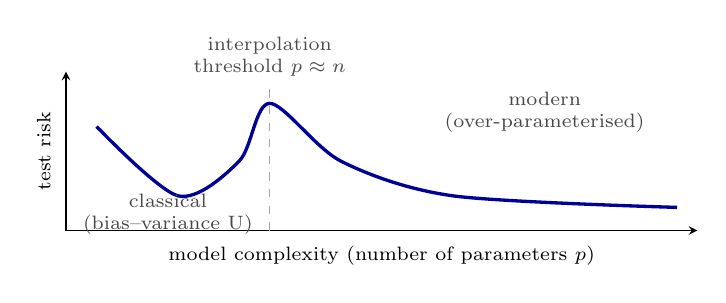
\begin{tikzpicture}
\begin{axis}[
  width=9.6cm, height=3.6cm,
  xlabel={\scriptsize model complexity (number of parameters $p$)},
  ylabel={\scriptsize test risk},
  xtick=\empty, ytick=\empty,
  xmin=0, xmax=3.1, ymin=0.5, ymax=3.25,
  axis lines=left, clip=false]
\draw[gray!70, dashed] (axis cs:1,0.5) -- (axis cs:1,3.0);
\node[gray!60!black, font=\scriptsize, anchor=south, align=center] at (axis cs:1,3.0) {interpolation\\ threshold $p\approx n$};
\addplot[blue!60!black, very thick, smooth] coordinates {(0.15,2.3)(0.55,1.1)(0.85,1.7)(1.0,2.7)(1.35,1.7)(1.9,1.1)(3.0,0.9)};
\node[font=\scriptsize, align=center, gray!55!black] at (axis cs:0.5,0.78) {classical\\ (bias--variance U)};
\node[font=\scriptsize, align=center, gray!55!black] at (axis cs:2.35,2.55) {modern\\ (over-parameterised)};
\end{axis}
\end{tikzpicture}
\end{center}
\vspace{-2mm}
\begin{itemize}\footnotesize\setlength{\itemsep}{0.8mm}
  \item \textbf{The interpolation threshold.} As $p$ grows, test risk follows the classical U --- until $p\approx n$, where the model fits the sample exactly and risk \textbf{peaks}.
  \item \textbf{The second descent.} Push past it, $p\gg n$: descent selects a \textbf{minimum-norm} interpolant, and test risk \emph{falls again}.
\end{itemize}
\begin{takeawaybox}\footnotesize
\textbf{More parameters than observations can help rather than hurt} --- which is not a licence to stop measuring, but is why the $1{,}377$-parameter network of 7.B1 is not absurd on a problem with no data at all.
\end{takeawaybox}
\vspace{1mm}
\src{Belkin, Hsu, Ma \& Mandal (2019), \emph{PNAS}.}
\end{frame}

%=============================================================================
\begin{frame}{Where the ``Implicit Regularisation'' Comes From}
\begin{columns}[T]
\begin{column}{0.54\textwidth}
\small
\textbf{Take the smallest case:} fit \textbf{two} points with \textbf{three} parameters. Infinitely many parameter vectors pass through both, the loss is zero at every one, and it cannot choose. \textbf{So what does?}
\smallskip

\textbf{The optimizer does, and its preference is the $\ell_2$ norm} --- of all exact fits, descent from zero returns the smallest-coefficient one: the \textbf{flattest} curve through the points.
\begin{itemize}\small\setlength{\itemsep}{0.6mm}
  \item In least squares, descent from the origin converges \emph{exactly} to the minimum-$\lVert w\rVert_2$ solution --- the pseudo-inverse $w=\Phi^{+}y$.
  \item In separable classification it converges in direction to the max-margin (again minimum-norm) predictor.
\end{itemize}
{\footnotesize \textbf{No penalty is ever written down} --- the dynamics of descent supply the bias.}
\end{column}
\begin{column}{0.43\textwidth}
\begin{conceptbox}[title=\textbf{The mechanism}]\footnotesize
From a near-zero start, descent only moves along directions the data excites. The ``wiggly'' null-space directions are never touched, so the solution stays small --- and small norm means \textbf{smooth}, which is what powers the second descent.
\medskip
\textbf{The analogy:} Tikhonov regularisation with $\lambda\to0^{+}$, selected by the algorithm rather than by you.
\end{conceptbox}
\end{column}
\end{columns}
\vspace{1mm}
\src{Soudry, Hoffer, Nacson, Gunasekar \& Srebro (2018). \textbf{Seen in \repo{labs/L07_ML_and_Deep_Growth.ipynb}{L07}}: descent on an under-determined fit lands on the minimum-norm point.}
\end{frame}

%=============================================================================
\begin{frame}{Why an Economist Should Care: the Blessings of Dimensionality}
\begin{columns}[T]
\begin{column}{0.49\textwidth}
\small
\textbf{In forecasting.} Liao, Ma, Neuhierl \& Shi (2023) ask whether noise hurts economic forecasts. When the target is driven by \emph{latent factors}, forecasting models are \textbf{not sparse}: adding many predictors --- \emph{even pure noise} --- past the sample size \emph{lowers} out-of-sample risk, beating PCA- and LASSO-style reduction on US inflation. Overfitting need not inflate out-of-sample variance.
\end{column}
\begin{column}{0.49\textwidth}
\small
\textbf{In solving models.} Ebrahimi Kahou \& Fern\'andez-Villaverde (2026) find the same double descent in networks that minimise \textbf{Euler and Bellman residuals}:
\begin{itemize}\small\setlength{\itemsep}{0.8mm}
  \item \textbf{no overfitting} --- as width grows, \emph{off-grid} residuals keep falling toward the benchmark solution;
  \item \textbf{algorithmic stability} --- wide networks concentrate across random seeds where narrow ones do not.
\end{itemize}
Measured on LQ, McCall and growth models.
\end{column}
\end{columns}
\medskip
\begin{takeawaybox}\footnotesize
\textbf{Over-parameterisation is a feature.} And note why the second result matters here: its ``no overfitting'' claim is about \textbf{off-grid Euler residuals} --- exactly the validation instrument 7.B3 insists on.
\end{takeawaybox}
\end{frame}

%=============================================================================
\begin{frame}{Takeaways, and What Is Still Missing}
\begin{columns}[T]
\begin{column}{0.54\textwidth}
\begin{takeawaybox}\small
\begin{itemize}\small\setlength{\itemsep}{1.1mm}
  \item Backpropagation is the chain rule with the intermediate quantities named and reused --- and those quantities are \textbf{shadow prices}.
  \item The optimizer is first-order because it must be: $10^{12}$ Hessian entries at $N=10^{6}$. \textbf{Adam is SGD with per-parameter steps.}
  \item What is guaranteed is a \emph{stationary point} under the Robbins--Monro conditions. 3.A2's contraction bound is gone.
  \item Measured here: a training loss \textbf{below the noise floor} is the overfitting diagnostic, and regularisation pays when data is scarce and almost nowhere else.
\end{itemize}
\end{takeawaybox}
\end{column}
\begin{column}{0.43\textwidth}
\begin{conceptbox}[title=\textbf{Bridge}]\small
You can now train a generic $\mathcal{N}(x;\theta)$ end to end. \textbf{Generic is not enough for economics.}
\medskip
\textbf{7.A4} asks which constraints on $\mathbf{W}$ a structured problem deserves; \textbf{7.B3} imposes the ones theory dictates --- monotonicity, convexity --- by construction rather than by hope.
\end{conceptbox}
\medskip
\begin{examplebox}\footnotesize
And Block B asks the question this deck has carefully avoided: what do you train on when \textbf{there is no dataset}?
\end{examplebox}
\end{column}
\end{columns}
\end{frame}

\end{document}
